% PartScribe technical report (Vietnamese). Build: xelatex main && xelatex main
\documentclass[11pt,a4paper]{article}
\usepackage{fontspec}
\setmainfont{Liberation Serif}
\setsansfont{Liberation Sans}
\setmonofont{Liberation Mono}[Scale=0.9]
\usepackage[margin=2.3cm]{geometry}
\usepackage{amsmath,amssymb}
\usepackage{graphicx}
\usepackage{booktabs,tabularx,multirow,array}
\usepackage{xcolor}
\usepackage{tikz}
\usetikzlibrary{positioning,arrows.meta,fit,backgrounds,calc}
\usepackage{caption,subcaption}
\usepackage{enumitem}
\usepackage{float}
\usepackage{placeins}
\usepackage[hidelinks]{hyperref}
\usepackage{microtype}
\setlist{itemsep=2pt,topsep=3pt}
\captionsetup{font=small,labelfont=bf}
\graphicspath{{figures/}}
\definecolor{nfd}{HTML}{1F6FB2}
\definecolor{chr}{HTML}{D9822B}
\definecolor{boxc}{HTML}{EEF4FA}
\newcommand{\pairok}{\texttt{pair\_ok}}
\newcommand{\note}[1]{\par\smallskip\noindent\fcolorbox{nfd!60}{boxc}{\parbox{0.97\linewidth}{\small #1}}\par\smallskip}
\renewcommand{\tablename}{Bảng}
\renewcommand{\figurename}{Hình}
\renewcommand{\contentsname}{Mục lục}
\renewcommand{\refname}{Tài liệu tham khảo}
\renewcommand{\abstractname}{Tóm tắt}
\renewcommand{\appendixname}{Phụ lục}

\title{\textbf{PartScribe: sinh chữ viết tay tiếng Việt theo phong cách người viết,\\ với nội dung biểu diễn bằng thành phần chữ}\\[4pt]
\large Báo cáo kỹ thuật chi tiết}
\author{Nhóm PartScribe}
\date{22/11/2026 \quad (nhánh \texttt{research/partscribe}, bản chốt \texttt{nfd v3 350k})}

\begin{document}
\maketitle

\begin{abstract}
Sinh chữ viết tay theo phong cách (\emph{styled handwritten text generation}, HTG) là bài toán tạo ảnh một từ hoặc cụm từ bất kỳ, nhìn như do \emph{một người cụ thể} viết, chỉ từ vài ảnh mẫu chữ của người đó. Với tiếng Việt, bài toán khó hơn tiếng Anh vì mỗi chữ cái có thể mang một hoặc hai dấu chồng lên nhau (ví dụ \emph{ễ} = \emph{e} + dấu mũ + dấu ngã), tạo ra 178 chữ cái khác nhau (89 thường, 89 hoa). Nhiều tổ hợp rất hiếm hoặc không hề có trong dữ liệu. Các mô hình hiện có coi mỗi ký tự là một đơn vị riêng, nên không thể viết một ký tự chưa từng thấy ảnh.

Báo cáo này trình bày \textbf{PartScribe}. Đây là mô hình khuếch tán tiềm ẩn kiểu \emph{rectified flow}, gồm một VAE, một Transformer khử nhiễu DiT và hai tầng biểu diễn phong cách. Điểm khác biệt là PartScribe biểu diễn nội dung bằng \textbf{thành phần chữ dùng chung} (chữ cái gốc, dấu biến đổi, dấu thanh theo phân rã Unicode NFD) thay vì một mã riêng cho mỗi ký tự. Chúng tôi xây dựng một \textbf{protocol giữ lại tổ hợp}: loại hẳn khỏi dữ liệu train mọi ảnh chứa 9 ký tự (\emph{è é ẻ ẹ ỷ ễ ỡ ử ẳ}), trong khi các thành phần của chúng vẫn xuất hiện ở ký tự khác. Sau đó đo xem mô hình có viết đúng các ký tự đó không. Phép đo dùng chỉ số đối chứng \pairok{} để loại bỏ việc OCR tự đoán dấu.

Trên 30 người viết chưa thấy khi train:
\begin{itemize}
\item Biểu diễn thành phần viết đúng ký tự giữ lại ở mức \textbf{0,823}, so với \textbf{0,006} khi dùng mã ký tự nguyên khối, trên cùng kiến trúc và dữ liệu.
\item Trên ký tự đã thấy, hai cách biểu diễn ngang nhau.
\item So với VATr++ huấn luyện cho tiếng Việt, PartScribe có FID 16,5 so với 38,5 và HWD 0,87 so với 1,61, tức giống ảnh thật và giống người viết hơn nhiều. VATr++ có tỉ lệ lỗi ký tự thấp hơn (1,2\% so với 2,8\%), nhưng thấp hơn cả ảnh thật (8,8\%).
\item Bổ sung dữ liệu chữ hoa có người viết thật giúp chữ hoa giống người viết hơn rõ rệt: HWD giảm từ 0,83 xuống 0,69 trên 5 người viết chưa thấy.
\end{itemize}
Báo cáo viết cho người \emph{chưa có kiến thức} về lĩnh vực này: mục~\ref{sec:background} giải thích mọi khái niệm nền trước khi vào phương pháp.
\end{abstract}

\tableofcontents
\newpage

%=====================================================================
\section{Giới thiệu}
\label{sec:intro}

\subsection{Bài toán}
Hãy tưởng tượng bạn có 15 tấm ảnh chụp chữ viết tay của một người, ví dụ \emph{``qua'', ``bảy'', ``cách''}. Bạn muốn máy tính viết thêm \emph{bất kỳ} từ nào khác (\emph{``Hà Nội'', ``Nguyễn'', ``trường học''}) sao cho trông như chính người đó viết: cùng độ nghiêng, cùng độ đậm nét, cùng cách viết chữ \emph{g} hay dấu mũ. Đó là bài toán \textbf{sinh chữ viết tay theo phong cách} (HTG). Hình~\ref{fig:teaser} minh họa đầu vào và đầu ra.

\begin{figure}[t]
\centering
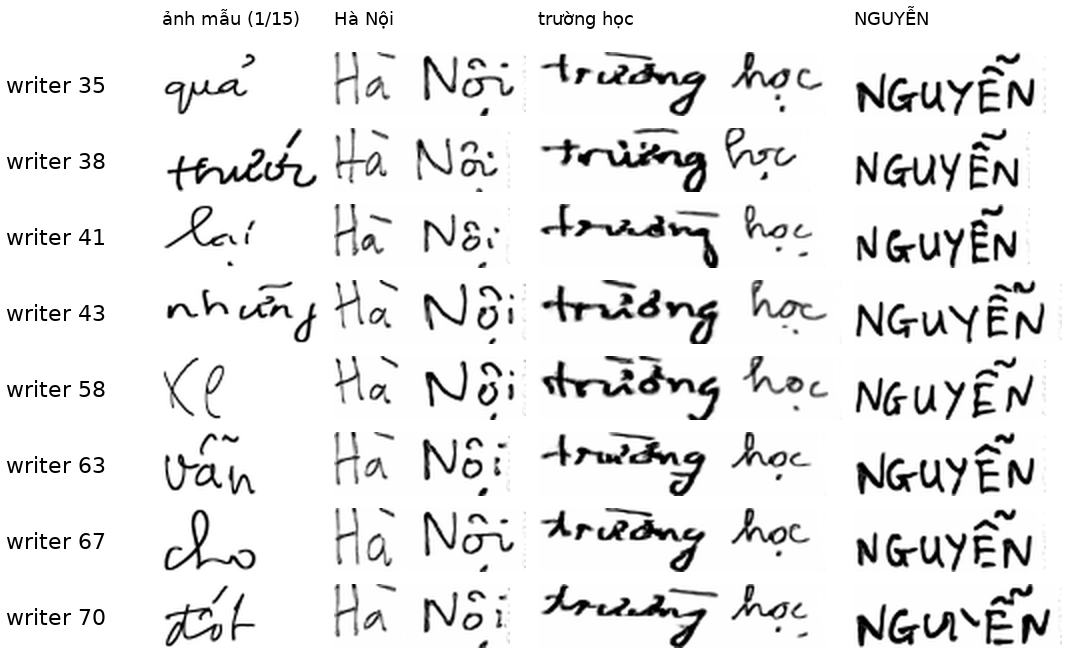
\includegraphics[width=\linewidth]{styles.png}
\caption{Đầu vào và đầu ra của PartScribe (bản chốt). Mỗi hàng là một người viết \emph{chưa từng xuất hiện khi train}. Cột đầu là 1 trong 15 ảnh mẫu (support) của người đó; các cột sau là chữ do mô hình sinh. Mô hình chưa từng thấy ảnh thật nào của các từ này do chính những người viết này viết.}
\label{fig:teaser}
\end{figure}

Ứng dụng gồm:
\begin{itemize}
\item tạo dữ liệu huấn luyện cho hệ nhận dạng chữ viết tay (OCR/HTR), đặc biệt cho ngôn ngữ ít dữ liệu;
\item điền biểu mẫu, phông chữ cá nhân hóa, hỗ trợ người khuyết tật vận động;
\item nghiên cứu khả năng tổ hợp (\emph{compositional generalisation}) của mô hình sinh.
\end{itemize}

\subsection{Vì sao tiếng Việt khó}
Tiếng Việt dùng chữ Latinh nhưng thêm nhiều dấu (chi tiết ở mục~\ref{sec:viet}):
\begin{itemize}
\item \textbf{dấu biến đổi}: mũ (â ê ô), trăng (ă), móc (ơ ư), và chữ đ;
\item \textbf{5 dấu thanh}: huyền, sắc, hỏi, ngã, nặng.
\end{itemize}
Hai loại dấu có thể \emph{chồng lên nhau}: \emph{ễ, ỡ, ử, ẳ, Ộ}. Kết quả là 178 chữ cái (89 thường, 89 hoa), trong đó 67 chữ hoa có dấu. Phân bố tần suất của chúng rất lệch (Hình~\ref{fig:longtail}):
\begin{itemize}
\item chữ \emph{n} xuất hiện hàng chục nghìn lần;
\item \textbf{42 chữ hoa có dấu (Ễ, Ê, Ộ, \dots) xuất hiện 0 lần} trong dữ liệu huấn luyện tiếng Việt.
\end{itemize}

\begin{figure}[t]
\centering
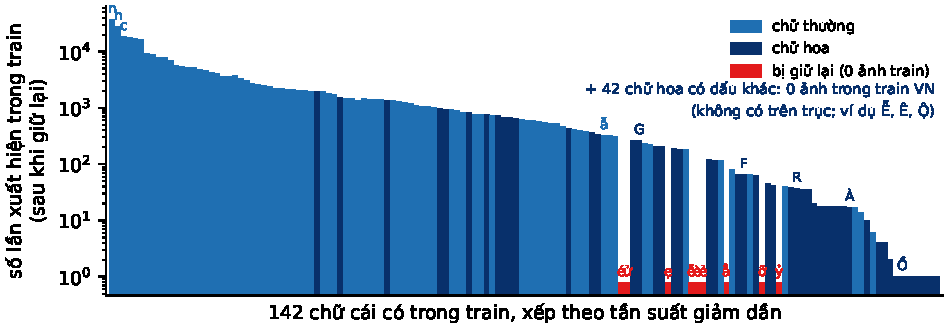
\includegraphics[width=\linewidth]{char_longtail.pdf}
\caption{Đuôi dài (long tail) của chữ cái trong tập train tiếng Việt (96.374 ảnh từ, 265 người viết), trục tung theo thang log. Thanh đỏ là các ký tự bị giữ lại theo protocol (0 ảnh train). Ngoài 142 chữ cái có mặt, còn 42 chữ hoa có dấu hoàn toàn vắng mặt.}
\label{fig:longtail}
\end{figure}

Các mô hình HTG phổ biến biểu diễn mỗi ký tự bằng một vector riêng (\emph{embedding}), hoặc bằng ảnh glyph của ký tự đó trong một phông chữ. Nếu ký tự không có ảnh viết tay nào khi train, vector của nó không bao giờ được học. Mô hình sẽ viết sai, thường thay bằng một ký tự ``anh em'' (ví dụ \emph{Ê} thay cho \emph{Ễ}).

\subsection{Ý tưởng chính và đóng góp}
Người Việt viết \emph{ễ} bằng cách viết \emph{e}, thêm dấu mũ, rồi thêm dấu ngã. Nếu mô hình học được từng \emph{thành phần} từ các ký tự khác (\emph{e} từ ``e'', dấu mũ từ ``ê'', dấu ngã từ ``ẽ, ỗ''), nó có thể \emph{ghép} ra \emph{ễ} dù chưa từng thấy ảnh \emph{ễ}. Đóng góp của báo cáo:
\begin{enumerate}
\item \textbf{PartScribe}: một mô hình HTG khuếch tán tiềm ẩn. Nội dung được biểu diễn bằng thành phần chữ; phong cách đi qua hai tầng (toàn cục và cục bộ); bố cục ký tự được dự đoán tường minh (mục~\ref{sec:method}).
\item \textbf{Protocol giữ lại tổ hợp} có kiểm soát cho tiếng Việt (9 ký tự, 3 mức độ khó), khóa bằng mã băm trước khi train, kèm chỉ số \pairok{} chống thiên lệch của OCR (mục~\ref{sec:protocol}, \ref{sec:eval}).
\item \textbf{Kết quả định lượng}: so sánh với baseline mã ký tự nguyên khối (cùng kiến trúc) và với VATr++, trên ba trục: ký tự giữ lại, chất lượng chung, chữ hoa của người viết thật (mục~\ref{sec:results}).
\item \textbf{Phân tích}:
  \begin{itemize}
  \item kết quả null của việc học thành phần không nhãn;
  \item thiên lệch của OCR khi chấm dấu;
  \item lỗi giải mã ở mép ảnh và cách sửa;
  \item các giới hạn còn lại (mục~\ref{sec:analysis}, \ref{sec:limits}).
  \end{itemize}
\end{enumerate}

%=====================================================================
\section{Kiến thức nền cho người mới}
\label{sec:background}
Mục này giải thích mọi khái niệm cần để đọc phần sau. Người đã quen với mô hình khuếch tán có thể bỏ qua.

\subsection{Ảnh chữ viết tay, ``người viết'' và ``phong cách''}
\begin{itemize}
\item Mỗi mẫu dữ liệu là một \textbf{ảnh xám} của \emph{một từ}, kèm \textbf{nhãn văn bản} (transcript) và \textbf{mã người viết} (writer ID).
\item Ở tiếng Việt, mọi ảnh được chuẩn hóa về \textbf{cao 32 pixel}; chiều rộng thay đổi theo độ dài từ.
\item \textbf{Phong cách} (style) là mọi thứ khiến chữ của hai người khác nhau khi viết cùng một từ: độ nghiêng, độ dày nét, cỡ chữ, khoảng cách, nét nối, hình dạng dấu.
\item Mô hình nhận phong cách qua \textbf{ảnh mẫu (support)}: 15 ảnh từ \emph{khác} của cùng người viết.
\end{itemize}

\textbf{Một số thuật ngữ:}
\begin{itemize}
\item \textbf{Few-shot}: chỉ cần vài ảnh mẫu của người viết mới, không cần train lại mô hình.
\item \textbf{Người viết chưa thấy} (unseen writer): người không có ảnh nào trong tập train. Mọi đánh giá trong báo cáo dùng người viết chưa thấy.
\item \textbf{Offline} và \textbf{online}: offline là ảnh tĩnh (như ảnh scan); online là chuỗi tọa độ nét bút. PartScribe làm việc với ảnh offline.
\end{itemize}

\subsection{Chữ Việt, Unicode và phân rã NFD}
\label{sec:viet}
Máy tính lưu chữ \emph{ễ} theo hai cách tương đương:
\begin{itemize}
\item \textbf{NFC}: một mã duy nhất (U+1EC5);
\item \textbf{NFD}: ba mã, gồm \emph{e} (U+0065), dấu mũ tổ hợp (U+0302) và dấu ngã tổ hợp (U+0303).
\end{itemize}
Phép biến đổi NFC $\to$ NFD có sẵn trong mọi ngôn ngữ lập trình (\texttt{unicodedata.normalize}). Bảng~\ref{tab:nfd} cho thấy cách PartScribe dùng NFD để tách ký tự thành tối đa 3 ``khe'' (slot).

\begin{table}[h]
\centering\small
\caption{Phân rã ký tự thành thành phần (chế độ \texttt{nfd}). Mỗi thành phần có embedding dùng chung cho mọi ký tự chứa nó.}
\label{tab:nfd}
\begin{tabular}{lllll}
\toprule
Ký tự & Khe 0: chữ gốc & Khe 1 & Khe 2 & Thành phần học được từ \\
\midrule
ễ & e (thường) & dấu mũ & dấu ngã & ê, ẽ, ỗ, ẫ \\
Ễ & e (\textbf{hoa}) & dấu mũ & dấu ngã & E, Ê, ỗ \dots{} (cờ hoa dùng chung) \\
ẹ & e (thường) & dấu nặng & -- & e, ạ, ọ, ụ \\
ử & u (thường) & dấu móc & dấu hỏi & ư, ở, ủ \\
ẳ & a (thường) & dấu trăng & dấu hỏi & ă, ả (cặp trăng + hỏi chưa từng có) \\
đ & đ (chữ riêng) & -- & -- & đ \\
\bottomrule
\end{tabular}
\end{table}

\subsection{Mạng nơ-ron, embedding và attention}
\begin{itemize}
\item \textbf{Embedding} là một vector số học được, đại diện cho một thực thể rời rạc (ký tự, dấu). Hai thực thể giống nhau có thể học ra hai vector gần nhau.
\item \textbf{Attention}: mỗi phần tử (\emph{query}) tính độ liên quan với các phần tử khác (\emph{key}), rồi lấy trung bình có trọng số của các \emph{value}. Self-attention là attention trong cùng một chuỗi. \textbf{Cross-attention} cho chuỗi này ``đọc'' thông tin từ chuỗi khác, ví dụ ảnh đọc nội dung văn bản.
\item \textbf{Transformer}: chồng nhiều lớp attention và mạng truyền thẳng (MLP) \cite{vaswani2017}.
\item \textbf{DiT} (Diffusion Transformer) \cite{peebles2023}: Transformer dùng để khử nhiễu ảnh. Ảnh được cắt thành các ô nhỏ (\emph{patch}), mỗi ô thành một token.
\end{itemize}

\subsection{VAE: nén ảnh vào không gian tiềm ẩn}
\textbf{VAE} (Variational Autoencoder) \cite{kingma2014} gồm hai phần:
\begin{itemize}
\item \emph{encoder} nén ảnh thành một tensor nhỏ hơn, gọi là \textbf{latent};
\item \emph{decoder} dựng lại ảnh từ latent.
\end{itemize}
Thay vì sinh trực tiếp pixel, mô hình sinh latent rồi giải mã. Cách này nhanh hơn và cho mô hình sinh tập trung vào cấu trúc thay vì chi tiết pixel. Đây là ý tưởng của \emph{latent diffusion} \cite{rombach2022}. PartScribe nén mỗi chiều 4 lần (hệ số $f=4$): ảnh $32\times W$ thành latent $4\times 8\times W/4$.

\subsection{Mô hình khuếch tán và rectified flow}
\label{sec:bg-flow}
\textbf{Ý tưởng:} học cách biến \emph{nhiễu ngẫu nhiên} thành \emph{dữ liệu}, từng bước nhỏ một \cite{ho2020}.
\begin{itemize}
\item \textbf{Huấn luyện}: lấy dữ liệu thật $x_0$, trộn với nhiễu $\varepsilon$ ở mức $t$, rồi dạy mạng đoán hướng cần đi.
\item \textbf{Sinh}: bắt đầu từ nhiễu, đi ngược dần về dữ liệu.
\end{itemize}

\textbf{Rectified flow} \cite{liu2023flow,lipman2023} là biến thể đơn giản: điểm trung gian nằm trên \emph{đường thẳng} nối dữ liệu và nhiễu,
\begin{equation}
x_t = (1-t)\,x_0 + t\,\varepsilon,\qquad t\in[0,1],\qquad v^\star = \varepsilon - x_0 .
\label{eq:rf}
\end{equation}
Mạng $v_\theta(x_t,t,\text{điều kiện})$ học dự đoán \emph{vận tốc} $v^\star$ bằng sai số bình phương. Khi sinh, ta giải phương trình $\mathrm{d}x/\mathrm{d}t = v_\theta$ từ $t=1$ (nhiễu) về $t=0$ (dữ liệu) bằng phương pháp Euler: chia thành 50 bước nhỏ, mỗi bước cập nhật $x \leftarrow x + \Delta t\cdot v_\theta$.

Hình~\ref{fig:flow} minh họa: hàng trên là $x_t$ đã giải mã, hàng dưới là ước lượng ``ảnh sạch'' $\hat x_0 = x_t - t\,v_\theta$ ở từng bước.

\begin{figure}[t]
\centering
\begin{minipage}{0.3\linewidth}\centering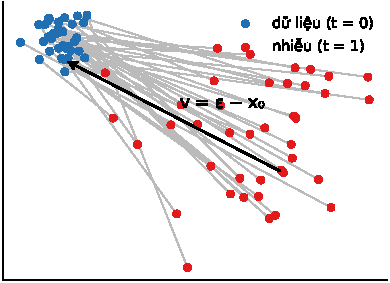
\includegraphics[width=\linewidth]{flow_schematic.pdf}\end{minipage}\hfill
\begin{minipage}{0.68\linewidth}\centering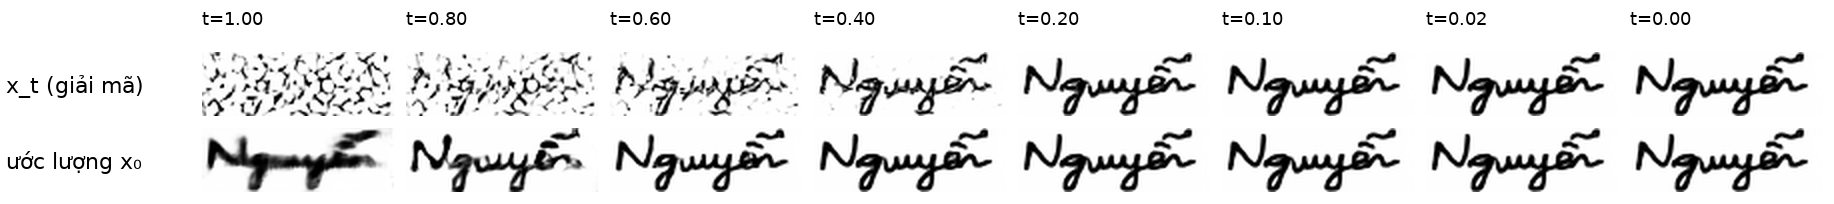
\includegraphics[width=\linewidth]{trajectory.png}\end{minipage}
\caption{Rectified flow. \textbf{Trái}: mỗi mẫu dữ liệu được nối với một mẫu nhiễu bằng đường thẳng; mạng học vận tốc dọc đường đó. \textbf{Phải}: quá trình sinh chữ ``Nguyễn'' thật của PartScribe, từ $t=1$ (nhiễu) tới $t=0$. Ngay từ $t\approx 0{,}8$, ước lượng $\hat x_0$ đã có hình dạng từ; các bước sau chủ yếu làm sắc nét.}
\label{fig:flow}
\end{figure}

\subsection{Classifier-free guidance (CFG)}
Để ảnh sinh ra \emph{bám sát điều kiện} (đúng chữ, đúng người viết), khi train ta thỉnh thoảng (10\%) bỏ điều kiện đi. Mạng vì vậy học được cả dự đoán có điều kiện lẫn không điều kiện. Khi sinh, ta khuếch đại hiệu giữa hai dự đoán \cite{ho2022cfg}:
\begin{equation}
v = v_\varnothing + w\,(v_{\text{cond}} - v_\varnothing),\qquad w>1 .
\end{equation}
PartScribe tách guidance cho \emph{nội dung} và \emph{phong cách} (mục~\ref{sec:sampling}), nên chỉnh được riêng ``đúng chữ'' và ``giống người viết''.

\subsection{Đo chất lượng chữ viết tay}
\label{sec:bg-metrics}
\begin{itemize}
\item \textbf{OCR} (nhận dạng chữ) và \textbf{CER}: dùng một mô hình đọc chữ \emph{độc lập} đọc ảnh sinh. CER (Character Error Rate) là số lần sửa ký tự tối thiểu (khoảng cách Levenshtein) chia cho độ dài từ. CER thấp nghĩa là chữ dễ đọc.
\item \textbf{FID} \cite{heusel2017} và \textbf{KID} \cite{binkowski2018}: đưa ảnh thật và ảnh sinh qua mạng InceptionV3, rồi đo khoảng cách giữa hai phân bố đặc trưng. Càng thấp, ảnh sinh càng giống ảnh thật \emph{về tổng thể}. \textbf{BFID} là FID trên ảnh đã nhị phân hóa (đen/trắng), bỏ qua khác biệt về màu nền.
\item \textbf{HWD} \cite{pippi2023hwd} (Handwriting Distance): đặc trưng lấy từ mạng VGG16 huấn luyện để phân biệt hơn 10.000 kiểu chữ viết. Tính trung bình đặc trưng ảnh sinh và ảnh thật \emph{của cùng một người viết}, lấy khoảng cách Euclid, rồi trung bình qua người viết. Càng thấp, chữ sinh càng \textbf{giống phong cách người viết}. Đây là chỉ số chính cho ``đúng phong cách''.
\item \textbf{Khoảng tin cậy (CI) bootstrap theo người viết}: lấy mẫu lại có hoàn lại danh sách người viết 1.000--2.000 lần, tính lại chỉ số, lấy phân vị 2,5\% và 97,5\%. Nếu CI của một hiệu số không chứa 0 thì khác biệt có ý nghĩa.
\end{itemize}

\subsection{Các công trình liên quan}
\begin{itemize}
\item \textbf{GAN}: HWT \cite{bhunia2021hwt} và \textbf{VATr / VATr++} \cite{pippi2023vatr,vanherle2024vatrpp} dùng Transformer và GAN. VATr biểu diễn ký tự bằng ảnh glyph phông Unifont (``visual archetype''), nên viết được \emph{một số} ký tự hiếm; ký tự vẫn là đơn vị nguyên khối. VATr++ là baseline chính của chúng tôi, đã được huấn luyện cho tiếng Việt trong dự án.
\item \textbf{Khuếch tán và tự hồi quy}: DiffusionPen \cite{nikolaidou2024}, One-DM \cite{dai2024onedm}, Emuru \cite{pippi2025emuru}, InkSpire \cite{inkspire2026}. InkSpire trộn style và nội dung trong một DiT, gần nhất về cơ chế. Các công trình này chỉ kiểm tra \emph{từ} chưa thấy, không kiểm tra \emph{ký tự hoặc tổ hợp dấu} chưa thấy có đối chứng.
\item \textbf{Chữ viết online}: SDT \cite{dai2023sdt}.
\item \textbf{Phông chữ theo thành phần} (Hán, Hàn): MX-Font và các biến thể dùng style theo bộ thủ, nhưng làm trên phông chữ in, không phải chữ viết tay của từng người.
\end{itemize}

%=====================================================================
\section{Bài toán và protocol giữ lại tổ hợp}
\label{sec:protocol}

\subsection{Định nghĩa}
\begin{itemize}
\item \textbf{Đầu vào}: chuỗi văn bản $y$ (một hoặc vài từ) và tập $S=\{s_1,\dots,s_{15}\}$ gồm 15 ảnh của một người viết $w$. Không ảnh nào trong $S$ có cùng nội dung với $y$.
\item \textbf{Đầu ra}: ảnh $\hat x$ cao 32 px, đọc ra đúng $y$ và mang phong cách của $w$.
\item \textbf{Đánh giá}: trên người viết \emph{không có trong tập train}.
\end{itemize}

\subsection{Protocol v1}
Để đo khả năng tổ hợp một cách sạch, chúng tôi \textbf{chọn trước} 9 ký tự, \textbf{loại toàn bộ ảnh và văn bản chứa chúng khỏi dữ liệu train}, và \textbf{khóa danh sách bằng mã băm SHA-256} trước khi train. Loader dữ liệu kiểm tra mã băm này ở mỗi lần chạy; mọi run ghi mã vào cấu hình.

\begin{table}[h]
\centering\small
\caption{Protocol giữ lại tổ hợp v1. ``Thành phần vẫn còn'' cho biết mô hình có thể học từng mảnh từ đâu.}
\label{tab:protocol}
\begin{tabularx}{\linewidth}{llX}
\toprule
Nhóm & Ký tự & Ý nghĩa và thành phần vẫn còn trong train \\
\midrule
C1 & è é ẻ ẹ ỷ & Dấu thanh đã thấy trên nguyên âm khác, đặt lên \emph{thân chữ mới} (ví dụ dấu nặng có ở ạ, ọ, ụ nhưng chưa từng trên e). \\
C2 & ễ ỡ ử & \emph{Cặp dấu chồng} đã thấy trên thân khác: mũ + ngã có ở ỗ, ẫ (657 ảnh); móc + ngã ở ữ (759); móc + hỏi ở ở. \\
C3 & ẳ & Cặp trăng + hỏi \emph{chưa từng xuất hiện ở bất kỳ ký tự nào} (thăm dò, mẫu nhỏ). \\
C4 & 42 chữ hoa có dấu & Không có ảnh thật tự nhiên trong dữ liệu VN; đo bằng tập chữ hoa riêng (mục~\ref{sec:c4}). \\
\bottomrule
\end{tabularx}
\end{table}

\textbf{Những gì được và không được thấy ký tự giữ lại:}
\begin{itemize}
\item Ảnh và transcript dùng để train generator: \textbf{không}.
\item Dữ liệu phụ (HAT2023, PNL): \textbf{không}, và loại \emph{cả dạng hoa} (È, Ễ\dots), chặt hơn protocol gốc.
\item \textbf{Bộ chấm OCR độc lập}: \emph{có} được train trên dữ liệu đầy đủ, vì nó chỉ dùng để chấm, không truyền gradient cho generator.
\end{itemize}

\textbf{Tiêu chí quyết định, khai báo trước:} biểu diễn thành phần phải hơn biểu diễn nguyên khối ít nhất 10 điểm phần trăm trên C1 $\cup$ C2, và CI 95\% của hiệu số không chứa 0.

%=====================================================================
\section{Phương pháp: PartScribe}
\label{sec:method}

\subsection{Tổng quan}
Hình~\ref{fig:arch} là sơ đồ toàn bộ mô hình, gồm 5 khối:
\begin{itemize}
\item \textbf{[E] VAE} nén và giải nén ảnh;
\item \textbf{[A+B] mã hóa nội dung} biến văn bản thành token;
\item \textbf{bộ dự đoán độ rộng} xác định mỗi ký tự chiếm bao nhiêu cột ảnh;
\item \textbf{[C] mã hóa phong cách} biến 15 ảnh mẫu thành vector $g$ và bộ nhớ $M$;
\item \textbf{[D] DiT} khử nhiễu latent dưới ba nguồn điều kiện.
\end{itemize}
Tổng cộng generator có \textbf{48,5 triệu tham số}:

\begin{center}\small
\begin{tabular}{lr}
\toprule
Khối & Tham số \\
\midrule
Nội dung & 7,1 triệu \\
Phong cách & 9,1 triệu \\
Dự đoán độ rộng & 0,3 triệu \\
DiT & 31,9 triệu \\
\midrule
\textbf{Tổng (generator)} & \textbf{48,5 triệu} \\
VAE (riêng) & 6,6 triệu \\
\bottomrule
\end{tabular}
\end{center}

\begin{figure}[t]
\centering
\resizebox{\linewidth}{!}{%
\begin{tikzpicture}[font=\small, node distance=6mm and 8mm,
  blk/.style={draw, rounded corners=2pt, minimum height=8mm, align=center, fill=white},
  inp/.style={draw, dashed, rounded corners=2pt, minimum height=7mm, align=center, fill=gray!8},
  arr/.style={-{Stealth[length=2mm]}, thick}]
\node[inp] (txt) {văn bản\\``Nguyễn''};
\node[blk, right=of txt, fill=nfd!12] (cont) {[A] token thành phần\\(NFD: chữ gốc, dấu, thanh)};
\node[blk, right=of cont, fill=nfd!12] (ctx) {[B] Context encoder\\Transformer 4 lớp};
\node[blk, below=of ctx, fill=nfd!6] (wid) {WidthHead\\độ rộng từng ký tự};
\node[inp, below=18mm of txt] (sup) {15 ảnh mẫu\\của người viết};
\node[blk, right=of sup, fill=chr!15] (sty) {[C] Style encoder\\CNN + 4 query};
\node[blk, below=5mm of sty, fill=chr!8] (M) {$M$: bộ nhớ patch\\(1.440 token)};
\node[blk, right=of sty, fill=chr!8] (g) {$g$: style toàn cục\\(SupCon, chống nội dung)};
\node[inp, below=of M] (noise) {nhiễu $z_1\!\sim\!\mathcal N(0,I)$, thời điểm $t$};
\node[blk, minimum height=30mm, minimum width=26mm, fill=nfd!20, right=22mm of wid] (dit) {[D] DiT\\8 block\\384 chiều\\[2pt]\scriptsize self-attn\\\scriptsize cross-attn nội dung\\\scriptsize cross-attn $M$\\\scriptsize AdaLN($t{+}g$)};
\node[blk, right=of dit] (euler) {Euler\\50 bước\\+ CFG};
\node[blk, right=of euler, fill=gray!10] (dec) {[E] VAE\\decoder};
\node[inp, right=of dec] (out) {ảnh\\32 px};
\draw[arr] (txt) -- (cont); \draw[arr] (cont) -- (ctx);
\draw[arr] (ctx) -- (wid);
\draw[arr] (ctx.east) -| node[pos=0.25, above, font=\scriptsize]{token nội dung} ($(dit.north)+(-6mm,0)$);
\draw[arr] (wid.east) -- node[above, font=\scriptsize]{bố cục} (wid.east -| dit.west);
\draw[arr] (sup) -- (sty); \draw[arr] (sty) -- (g); \draw[arr] (sty) -- (M);
\draw[arr] (g.east) -| ($(dit.south)+(6mm,0)$);
\draw[arr] (g) -- (wid);
\draw[arr] (M.east) -| ($(dit.south)$);
\draw[arr] (noise.east) -| ($(dit.south)+(-6mm,0)$);
\draw[arr] (dit) -- node[above, font=\scriptsize]{$v_\theta$} (euler); \draw[arr] (euler) -- node[above, font=\scriptsize]{$z_0$} (dec); \draw[arr] (dec) -- (out);
\end{tikzpicture}}
\caption{Kiến trúc PartScribe. Màu xanh là đường đi của nội dung; màu cam là đường đi của phong cách. VAE (xám) được train trước và đóng băng.}
\label{fig:arch}
\end{figure}

\subsection{[E] VAE cho ảnh chữ}
\begin{itemize}
\item \textbf{Biểu diễn ảnh}: ảnh được chuyển thành \textbf{bản đồ mực} trong $[0,1]$ (mực = 1, giấy = 0). Nhờ vậy vùng đệm bằng 0 chính là ``giấy trắng'', và ảnh rộng khác nhau xếp được vào cùng một batch.
\item \textbf{Kiến trúc}: encoder gồm hai lớp tích chập bước 2, cho ra latent 4 kênh. Decoder đối xứng, đầu ra qua sigmoid.
\item \textbf{Hàm mất mát}:
  \begin{itemize}
  \item L1 chỉ trên các cột hợp lệ;
  \item L1 trên biên nét (lọc Sobel), để nét sắc;
  \item KL rất nhỏ ($10^{-6}$);
  \item PatchGAN hinge loss (trọng số 0,05), bật sau 20.000 bước.
  \end{itemize}
\item \textbf{Huấn luyện}: 100.000 bước, batch 64, lr $2\cdot10^{-4}$.
\item \textbf{Chuẩn hóa latent}: sau khi train, đo độ lệch chuẩn của latent (2,41) và chia cho nó, để latent có phương sai xấp xỉ 1 như nhiễu Gauss.
\end{itemize}
Hình~\ref{fig:vae} cho thấy VAE tái tạo gần như hoàn hảo bên trong độ rộng chữ. Ở vùng đệm, nơi loss không giám sát, nó sinh rác. Vì vậy mọi ảnh sinh phải được che ngoài độ rộng dự đoán.

\begin{figure}[h]
\centering
\begin{minipage}{0.55\linewidth}\centering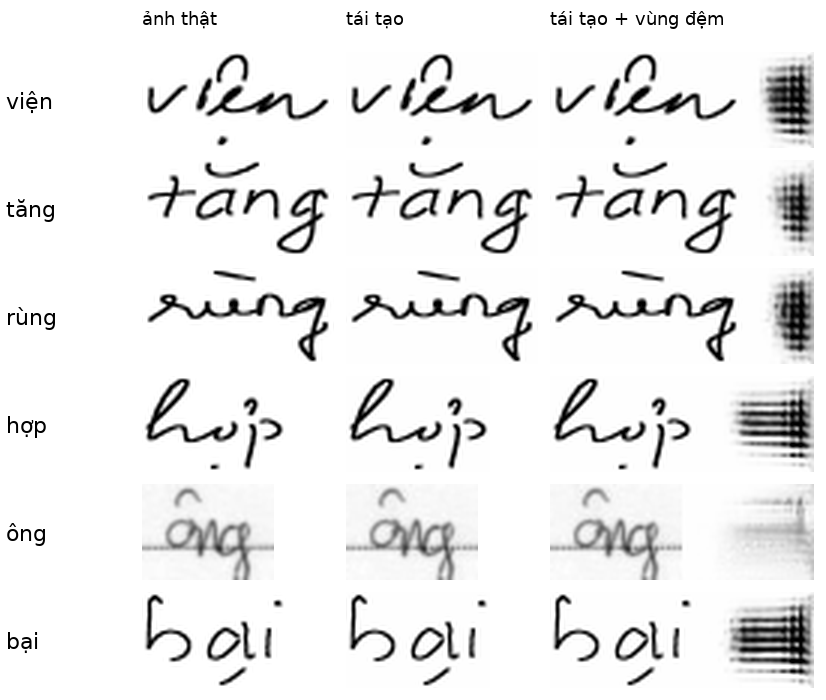
\includegraphics[width=\linewidth]{vae_recon.png}\end{minipage}\hfill
\begin{minipage}{0.42\linewidth}\centering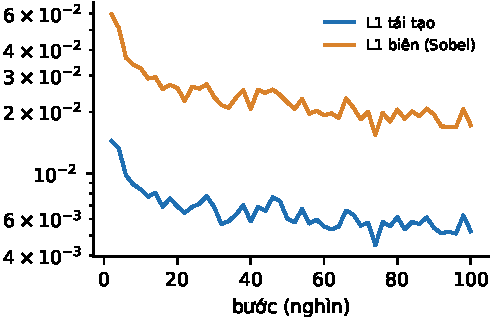
\includegraphics[width=\linewidth]{vae_curve.pdf}\end{minipage}
\caption{VAE tiếng Việt 32 px. \textbf{Trái}: ảnh thật, ảnh tái tạo trong độ rộng chữ, và tái tạo cả vùng đệm (rác ở bên phải). \textbf{Phải}: loss tái tạo khi train.}
\label{fig:vae}
\end{figure}

\subsection{[A] Biểu diễn nội dung: ba chế độ}
Bộ mã hóa nội dung có ba chế độ. Mọi phần khác của mô hình giữ nguyên, nên so sánh giữa các chế độ là công bằng.
\begin{description}
\item[\texttt{char} (baseline nguyên khối).] Mỗi ký tự một embedding riêng, 1 token mỗi ký tự. Ký tự bị giữ lại giữ nguyên embedding khởi tạo ngẫu nhiên, vì không có gì để học. Đây là hành vi ``trung thực'' của mọi mô hình coi ký tự là đơn vị nguyên khối.
\item[\texttt{nfd} (thành phần, nhánh chính).] Mỗi ký tự tối đa 3 token, như Bảng~\ref{tab:nfd}:
  \begin{itemize}
  \item token chữ gốc = $e_{\text{chữ}} + e_{\text{hoa/thường}} + e_{\text{vai trò}}$;
  \item token dấu = $e_{\text{dấu}} + e_{\text{vai trò}}$.
  \end{itemize}
  Khe không dùng bị che (mask). Mọi embedding dùng chung giữa các ký tự. Dấu cách là một token học được riêng.
\item[\texttt{parts} (thành phần học không nhãn, đã dừng).] Thành phần được học từ ảnh glyph phông chữ bằng Slot Attention \cite{locatello2020} và lượng tử hóa FSQ \cite{mentzer2024} (240 mã). Chế độ này đã thất bại ở bước kiểm tra trước (mục~\ref{sec:stage1}).
\end{description}

\subsection{[B] Context encoder}
\begin{itemize}
\item Token của mọi ký tự trong từ được xếp thành một chuỗi. Mỗi token được cộng mã vị trí theo \emph{chỉ số ký tự}, nên các token của cùng một ký tự có cùng vị trí.
\item Chuỗi đi qua một Transformer hai chiều: 4 lớp, 384 chiều, 6 đầu attention.
\item Nhờ vậy hình dạng một ký tự có thể phụ thuộc ký tự bên cạnh (nét nối, chữ hoa đầu từ).
\item Đầu ra gồm token nội dung cho DiT, và đặc trưng trung bình mỗi ký tự cho bộ dự đoán độ rộng.
\end{itemize}

\subsection{Dự đoán độ rộng và bố cục}
DiT không phải tự tìm ``chữ \emph{g} nằm ở cột nào''. Mô hình dự đoán độ rộng từng ký tự một cách \emph{tường minh}, giống bộ dự đoán thời lượng trong tổng hợp giọng nói:
\begin{equation}
w_i = \exp\big(\mathrm{MLP}([h_i;\,g])\big),\qquad c_i = \textstyle\sum_{j\le i} w_j - w_i/2 .
\end{equation}
\begin{itemize}
\item Độ rộng phụ thuộc người viết qua $g$: có người viết chữ rộng, có người viết chữ hẹp.
\item \textbf{Không có nhãn độ rộng từng ký tự}, chỉ biết tổng độ rộng ảnh. Vì vậy:
  \begin{itemize}
  \item loss độ rộng chỉ phạt sai số log của \emph{tổng};
  \item khi train, độ rộng dự đoán được co tỉ lệ cho khớp tổng thật;
  \item \emph{tỉ lệ} giữa các ký tự (\emph{i} hẹp, \emph{m} rộng) được học gián tiếp qua gradient của bias căn chỉnh (mục~\ref{sec:dit}).
  \end{itemize}
\end{itemize}

\subsection{[C] Phong cách hai tầng}
\begin{itemize}
\item Một CNN (bước tổng 8, 384 chiều) chạy trên từng ảnh mẫu; mỗi ảnh rộng tối đa 192 px.
\item \textbf{$M$ (bộ nhớ patch)}: toàn bộ đặc trưng của 15 ảnh trải phẳng, khoảng 1.440 token. $M$ \emph{cố ý} giữ thông tin cục bộ: DiT ``tra'' trong $M$ xem người này viết dấu mũ hay chữ \emph{g} thế nào.
\item \textbf{$g$ (style toàn cục)}: 4 query học được đọc từ $M$, lấy trung bình thành một vector 384 chiều. $g$ được ép thành ``danh tính người viết'' bằng hai loss:
  \begin{enumerate}
  \item \textbf{SupCon} \cite{khosla2020}: $g$ của cùng người viết gần nhau, khác người viết xa nhau. Batch gồm 16 người viết × 4 ảnh.
  \item \textbf{Chống mang nội dung}: một đầu phân loại cố đoán những chữ cái có trong ảnh mẫu từ $g$, nối qua \emph{gradient reversal} \cite{ganin2015}. Encoder bị đẩy ngược lại, để $g$ không ``nhớ'' nội dung.
  \end{enumerate}
\item Chống sao chép ở mức dữ liệu: ảnh mẫu không bao giờ chứa ảnh đích, hay ảnh có cùng transcript với đích.
\end{itemize}

\subsection{[D] DiT khử nhiễu}
\label{sec:dit}
Latent $4\times8\times W/4$ được cắt thành patch $2\times2$, mỗi patch thành một token 384 chiều, cộng mã vị trí 2D. Mỗi block thực hiện:
\begin{align*}
x &\leftarrow x + \gamma_1\cdot\mathrm{SelfAttn}(\mathrm{AdaLN}(x;\ t+g))\\
x &\leftarrow x + \alpha_c\odot\mathrm{CrossAttn}(x,\ \text{token nội dung};\ \text{bias } B)\\
x &\leftarrow x + \alpha_s\odot\mathrm{CrossAttn}(x,\ M)\\
x &\leftarrow x + \gamma_2\cdot\mathrm{MLP}(\mathrm{AdaLN}(x;\ t+g))
\end{align*}
\begin{itemize}
\item Mọi ``cổng'' ($\gamma,\alpha$, tham số AdaLN) khởi tạo bằng 0. Lúc đầu DiT là ánh xạ đồng nhất, và các nhánh điều kiện mở dần, giúp train ổn định.
\item \textbf{Bias căn chỉnh} $B$ (Hình~\ref{fig:align}): với cột ảnh $x$ và token thuộc ký tự $k$,
\begin{equation}
B(x,k) = -\tfrac12\Big(\frac{x-c_k}{\sigma_k}\Big)^2,\qquad \sigma_k = \tfrac{w_k}{2}\,\mathrm{softplus}(\tau) + 0{,}5 .
\end{equation}
Mỗi cột chủ yếu nhìn ký tự nằm dưới nó, nhưng vẫn thấy ký tự lân cận. Bias khả vi theo $w_k$, nên gradient từ loss khử nhiễu dạy luôn bộ dự đoán độ rộng.
\item Luôn có một \textbf{token rỗng} (null) trong ngữ cảnh nội dung và trong $M$. Nhờ vậy, khi bỏ điều kiện để làm CFG, attention vẫn có chỗ ``nhìn''.
\end{itemize}

\begin{figure}[h]
\centering
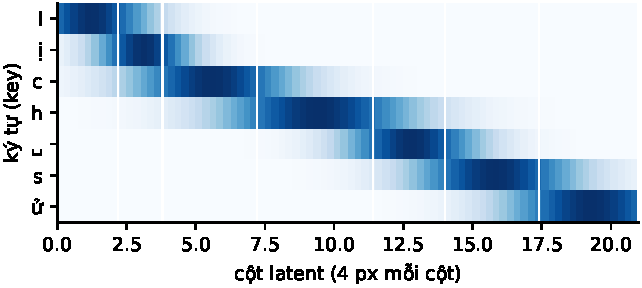
\includegraphics[width=0.7\linewidth]{align_bias.pdf}
\caption{Bias căn chỉnh của cross-attention nội dung cho từ ``lịch sử'' (minh họa). Mỗi hàng là một ký tự, mỗi cột là một cột latent; ô càng đậm, cột đó càng chú ý tới ký tự đó.}
\label{fig:align}
\end{figure}

\subsection{Hàm mất mát và huấn luyện}
\begin{equation}
\mathcal L = \underbrace{\mathbb E\,\big\|\,(v_\theta(x_t,t,c,g,M) - (\varepsilon-x_0))\odot m\,\big\|^2}_{\text{flow loss (chỉ cột hợp lệ, trọng số dấu)}} + 0{,}1\,\mathcal L_{\text{độ rộng}} + 0{,}05\,\mathcal L_{\text{SupCon}} + 0{,}05\,\mathcal L_{\text{chống nội dung}} .
\end{equation}
\begin{itemize}
\item \textbf{Lấy mẫu thời điểm}: $t$ lấy theo phân phối logit-normal \cite{esser2024}, dồn mẫu vào vùng giữa, nơi khó nhất.
\item \textbf{Trọng số dấu}: bản đồ $m$ nhân 4 tại các thành phần mực nhỏ (dấu, chấm), để loss không bị nét lớn áp đảo (mục~\ref{sec:sampler}).
\item \textbf{Classifier-free dropout}: bỏ nội dung 10\%, bỏ phong cách 10\%.
\item \textbf{Tối ưu}: AdamW, lr $10^{-4}$ cố định sau 5.000 bước khởi động, weight decay 0,01, cắt gradient 1,0, bf16.
\item \textbf{EMA}: trọng số trung bình trượt 0,9999, có giai đoạn khởi động.
\end{itemize}

\subsection{Sinh ảnh}
\label{sec:sampling}
Mỗi bước Euler chạy DiT ba lần trong cùng một batch (không điều kiện, chỉ nội dung, đầy đủ), rồi kết hợp:
\begin{equation}
v = v_\varnothing + w_c\,(v_{\text{nội dung}} - v_\varnothing) + w_s\,(v_{\text{đầy đủ}} - v_{\text{nội dung}}),\qquad w_c=3,\ w_s=1{,}5 .
\end{equation}
\begin{itemize}
\item Có thể thêm \emph{guidance dấu} $w_\text{mark}\,(v(y) - v(y_{\text{bỏ dấu}}))$, giữ nguyên bố cục.
\item Độ rộng ảnh sinh bằng tổng độ rộng dự đoán.
\item Latent được giải mã bằng \texttt{decode\_generated}: che ngoài độ rộng, rồi xóa vạch biên (mục~\ref{sec:edge}).
\end{itemize}

%=====================================================================
\section{Dữ liệu và chiến lược huấn luyện}
\label{sec:data}

\subsection{Nguồn dữ liệu}
\begin{table}[h]
\centering\small
\caption{Dữ liệu sử dụng. Tập test VN được niêm phong; mọi số trong báo cáo dùng tập val.}
\label{tab:data}
\begin{tabularx}{\linewidth}{lXr}
\toprule
Nguồn & Vai trò & Số lượng \\
\midrule
VNOnDB + ViHTGen (gộp theo VATr-pp) & Ảnh từ có người viết. Train: 265 người; val: 30 người khác hẳn & 96.374 ảnh train \\
HAT2023 & Ảnh không có mã người viết; dùng làm \emph{đích chỉ có nội dung}, 16 ảnh mỗi batch & 98.421 ảnh \\
PNL handwriting\_word\_v1.0 (từ v3) & Chữ hoa có người viết thật. Train: 14 người; test chữ hoa: 5 người & 4.623 / 1.653 ảnh \\
\bottomrule
\end{tabularx}
\end{table}

\paragraph{Chuẩn bị dữ liệu chữ hoa PNL.} Ảnh gốc 300 DPI được chuyển xám và thu về cao 32 px, giữ tỉ lệ. Hình học sau khi thu khớp với VNOnDB:

\begin{center}\small
\begin{tabular}{lcc}
\toprule
& PNL & VNOnDB \\
\midrule
Lề trên / dưới & 0,87 / 0,92 px & 0,87 / 0,90 px \\
Độ đậm nét (phân vị 90) & 0,96 & 0,99 \\
Tỉ lệ rộng/cao & 1,5 & 1,5 \\
\bottomrule
\end{tabular}
\end{center}

\begin{itemize}
\item \textbf{Lọc}: loại 1.155 ảnh chứa ký tự giữ lại (ở bất kỳ dạng hoa hay thường) và 169 ảnh bị gắn cờ chất lượng.
\item \textbf{Chia theo người viết}: 14 người để train, phủ \textbf{đủ 80/80 chữ hoa} mà protocol cho phép. 5 người còn lại không bao giờ dùng để train.
\end{itemize}
Hình~\ref{fig:pnl} cho một số mẫu.

\begin{figure}[h]
\centering
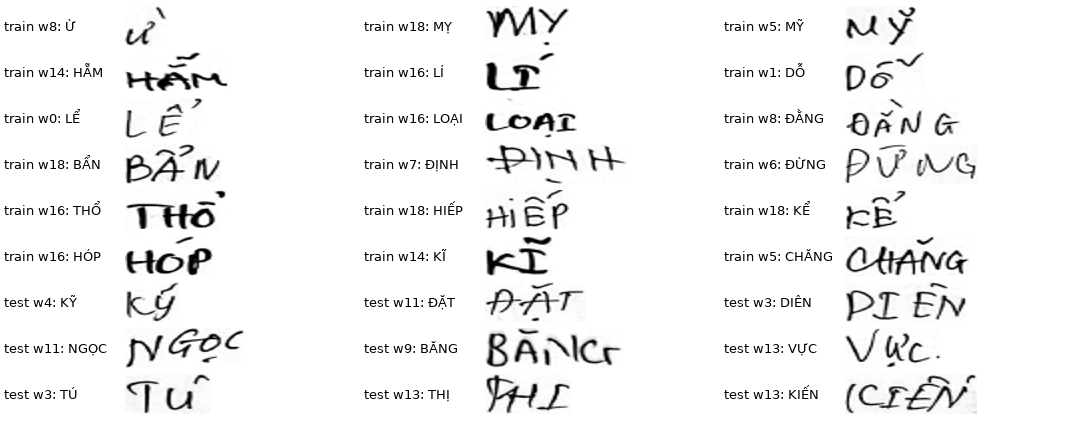
\includegraphics[width=0.9\linewidth]{pnl32_samples.png}
\caption{Dữ liệu chữ hoa PNL sau khi chuẩn hóa về 32 px (train: 14 người viết; test: 5 người viết khác).}
\label{fig:pnl}
\end{figure}

\subsection{Chiến lược lấy batch}
\label{sec:sampler}
Mỗi batch gồm 16 người viết × 4 ảnh đích, mỗi ảnh có 15 ảnh mẫu.
\begin{enumerate}
\item \textbf{Cân bằng nguồn}: chọn nguồn dữ liệu trước, rồi chọn người viết đều trong nguồn, để nguồn lớn không lấn át.
\item \textbf{Long-tail sampler} (chuyển từ VATr-pp): 30\% số lượt chọn ảnh ưu tiên ký tự và thành phần hiếm, với trọng số $\sqrt{N/\text{tần suất}}$.
\item \textbf{Ghép nhiều từ} (multiword, $p=0{,}2$): ghép 2--3 từ của \emph{cùng người viết} thành một cụm có dấu cách. Lý do: dữ liệu gần như không có dấu cách (109 trên 96.000 nhãn). Mọi từ được đặt trên \textbf{cùng một đường chân chữ}, rồi thu cả dòng về 32 px với một tỉ lệ chung.
\item \textbf{Trọng số dấu} (= 3): thành phần mực nhỏ (diện tích $\le 2{,}5\%\cdot h^2$, cao $\le 30\%\cdot h$) được nhân trọng số $1+3$ trong loss.
\item \textbf{HAT2023 làm đích chỉ có nội dung}: với các ảnh này, luôn bỏ phong cách, bộ dự đoán độ rộng dùng $g$ rỗng, và không tính SupCon hay loss chống nội dung.
\item \textbf{PNL} (v3): chiếm 15\% số lượt chọn người viết (đo thực tế 14,7\% đích thật).
\end{enumerate}

\subsection{Lịch sử các lần train}
\begin{table}[h]
\centering\small
\caption{Các run tiếng Việt (mỗi run gồm hai nhánh \texttt{char} và \texttt{nfd}, cấu hình giống hệt nhau).}
\label{tab:runs}
\begin{tabularx}{\linewidth}{lllX}
\toprule
Run & Bước & Khởi tạo & Thay đổi và lý do \\
\midrule
tự nhiên & 0--25k & ngẫu nhiên & Lấy mẫu theo tần suất tự nhiên; giữ làm ablation \\
\texttt{\_lt} & 0--100k & ngẫu nhiên & Long-tail sampler của VATr-pp \\
\texttt{v2a} & 100--110k & \texttt{\_lt} 100k & Ghép từ và trọng số dấu, nhưng ghép lệch dòng (mỗi từ chuẩn hóa riêng) $\Rightarrow$ dừng \\
\texttt{v2} & 100--200k & \texttt{\_lt} 100k & Ghép trên cùng đường chân chữ; HAT2023 làm đích chỉ có nội dung; tải batch song song \\
\texttt{v2} (tiếp) & 200--300k & \texttt{v2} 200k & Loss còn giảm; seed dữ liệu mới, lr giữ nguyên \\
\texttt{v3} & 300--400k & \texttt{v2} 300k & + dữ liệu chữ hoa PNL (15\%). \textbf{Chốt ở 350k} \\
\bottomrule
\end{tabularx}
\end{table}

\begin{figure}[h]
\centering
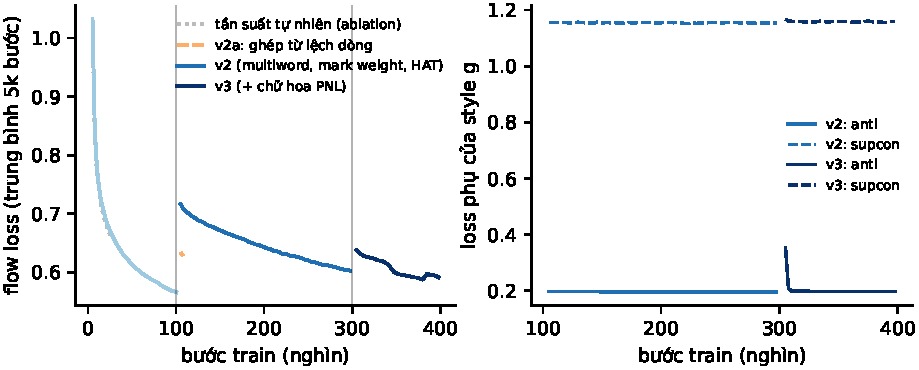
\includegraphics[width=\linewidth]{training_curves.pdf}
\caption{\textbf{Trái}: flow loss (trung bình trượt 5.000 bước) của nhánh \texttt{nfd} qua các run. Loss tăng nhẹ khi thêm dữ liệu mới ở 100k (ghép từ, HAT) và 300k (PNL), rồi giảm tiếp. \textbf{Phải}: hai loss phụ của $g$. Loss chống nội dung tăng vọt khi gặp 14 người viết PNL mới, rồi về lại mức cũ sau khoảng 10.000 bước.}
\label{fig:train}
\end{figure}

\paragraph{Tài nguyên tính toán.} Một GPU NVIDIA H200 dùng chung, hai nhánh char/nfd chạy song song. Tốc độ khoảng 12.000 bước/giờ mỗi nhánh khi GPU rảnh, khoảng 3.000--4.000 bước/giờ khi GPU bị chia. Cả quá trình 400.000 bước mất khoảng 4 ngày tính theo thời gian thực.

%=====================================================================
\section{Phương pháp đánh giá}
\label{sec:eval}

\subsection{Bộ chấm OCR độc lập và thiên lệch ``tự điền dấu''}
Bộ chấm OCR được train trên dữ liệu train đầy đủ, không bao giờ thấy tập val hay test, và tách biệt khỏi mọi mô hình sinh.

Chúng tôi phát hiện OCR loại CRNN + BiLSTM \cite{shi2017crnn} \textbf{tự điền dấu từ ngữ cảnh}. Phép thử như sau: \emph{xóa vùng dấu} trên ảnh thật, rồi cho OCR đọc lại.
\begin{itemize}
\item Với chữ \emph{mẹ} đã bị xóa dấu nặng, OCR vẫn đọc ra \emph{ẹ} 19/32 lần (Hình~\ref{fig:ocrgate}).
\item Một OCR như vậy sẽ chấm ``đúng'' cho ảnh sinh thiếu dấu, làm kết quả bị thổi phồng.
\end{itemize}
Chúng tôi thiết kế \textbf{LocalOCR}: các lớp tích chập cuối chỉ chạy theo chiều cao, không có hồi quy, nên mỗi cột đầu ra chỉ nhìn khoảng 29 px. Thiên lệch giảm nhưng chưa hết (12/32), vì vậy chỉ số chính dùng \pairok{}.

\begin{figure}[h]
\centering
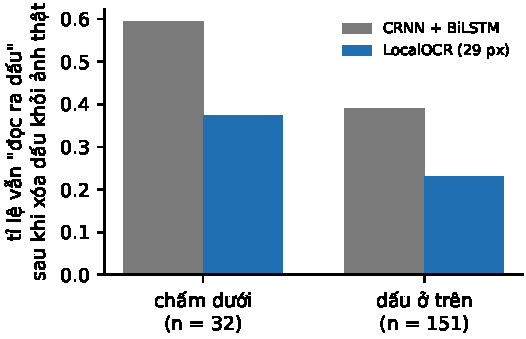
\includegraphics[width=0.45\linewidth]{ocr_gate.pdf}
\caption{Phép thử ``xóa dấu'': tỉ lệ OCR vẫn đọc ra dấu sau khi dấu đã bị xóa khỏi ảnh thật. Càng thấp càng trung thực.}
\label{fig:ocrgate}
\end{figure}

\subsection{Chỉ số cặp đối chứng \pairok}
Mỗi từ chứa ký tự giữ lại được sinh \textbf{hai lần}, dùng \emph{cùng nhiễu, cùng người viết, cùng bố cục}:
\begin{enumerate}
\item lần một với văn bản đầy đủ (\emph{mẹ});
\item lần hai với văn bản đã bỏ dấu (\emph{me}).
\end{enumerate}
Một vị trí được tính \textbf{đúng} khi bản có dấu đọc ra ký tự đích (\emph{ẹ}) \textbf{và} bản không dấu \emph{không} đọc ra ký tự đó. Nếu OCR tự điền dấu, nó sẽ đọc ra \emph{ẹ} ở cả hai bản và bị tính sai. Hình~\ref{fig:pairs} cho ví dụ thật.

\begin{figure}[h]
\centering
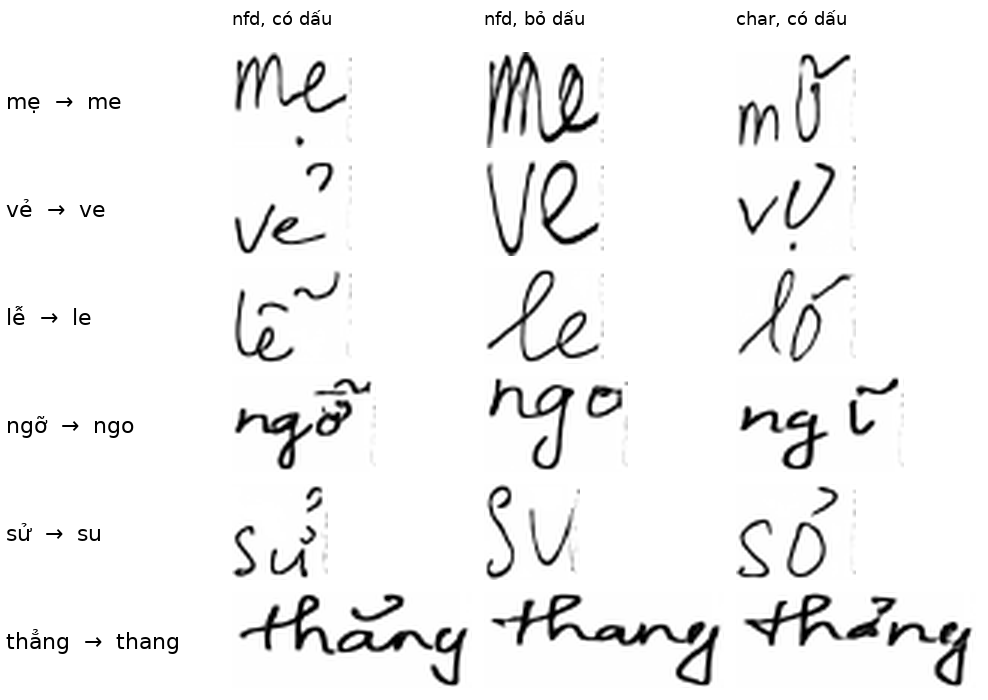
\includegraphics[width=0.8\linewidth]{pairs.png}
\caption{Cặp đối chứng do mô hình chốt sinh (một người viết val). Cột 1: \texttt{nfd} sinh từ có ký tự giữ lại. Cột 2: \texttt{nfd} sinh cùng từ đã bỏ dấu, cùng nhiễu và bố cục; khác biệt duy nhất là dấu. Cột 3: baseline \texttt{char} viết sai các ký tự chưa thấy (sai dấu hoặc mất dấu).}
\label{fig:pairs}
\end{figure}

\subsection{Metric chuẩn và các tập đánh giá}
\label{sec:c4}
\begin{description}
\item[Tập VN val.] 2.847 từ của 30 người viết val, chỉ gồm ký tự đã thấy. Mọi mô hình (kể cả VATr++) nhận \textbf{cùng từ đích và cùng 15 ảnh mẫu}. FID, KID, BFID và HWD tính theo đúng quy ước của repo HWD chính thức \cite{pippi2023hwd}. CER đo bằng OCR CRNN độc lập.
\item[Tập chữ hoa C4.] 1.653 từ chữ hoa của 5 người viết PNL không có trong train. Ảnh mẫu lấy từ chính chữ hoa của người đó.
\item[Khoảng tin cậy.] Bootstrap theo người viết; với so sánh cặp, lấy hiệu trên cùng người viết.
\end{description}

%=====================================================================
\section{Kết quả}
\label{sec:results}

\subsection{Ký tự giữ lại: khả năng tổ hợp}
\begin{table}[h]
\centering\small
\caption{Độ đúng trên ký tự giữ lại (30 người viết val). Các mốc đến 75k chấm bằng OCR CRNN (độ đúng thô); từ 100k chấm bằng LocalOCR và \pairok{}. CI là của hiệu \texttt{nfd} $-$ \texttt{char}.}
\label{tab:heldout}
\begin{tabular}{lcccccc}
\toprule
Mốc & \texttt{char} C1+C2 & \texttt{nfd} C1+C2 & CI 95\% hiệu & C1 & C2 & C3 \\
\midrule
tự nhiên 25k & 0,018 & 0,530 & +0,37..+0,60 & 0,51 & 0,56 & 0,68 \\
\texttt{\_lt} 75k & 0,018 & 0,848 & +0,71..+0,91 & 0,92 & 0,74 & 0,79 \\
\texttt{\_lt} 100k & 0,000 & 0,762 & +0,65..+0,84 & 0,77 & 0,76 & 0,63 \\
\texttt{v2} 200k & 0,000 & 0,805 & +0,72..+0,87 & 0,77 & 0,86 & 0,68 \\
\texttt{v2} 300k (sửa mép) & 0,012 & 0,829 & +0,75..+0,87 & 0,87 & 0,77 & 0,89 \\
\textbf{\texttt{v3} 350k (chốt)} & \textbf{0,006} & \textbf{0,823} & \textbf{+0,70..+0,88} & 0,83 & 0,82 & 0,84 \\
\texttt{v3} 400k & 0,012 & 0,774 & +0,67..+0,83 & 0,83 & 0,70 & 0,79 \\
\bottomrule
\end{tabular}
\end{table}

\begin{figure}[h]
\centering
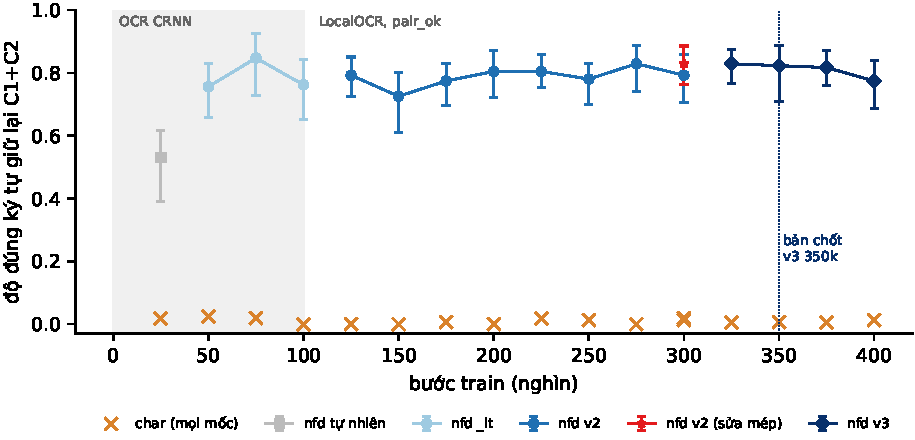
\includegraphics[width=\linewidth]{heldout_vs_steps.pdf}
\caption{Độ đúng ký tự giữ lại theo bước train, kèm CI 95\%. Dấu × là baseline \texttt{char}, luôn gần 0.}
\label{fig:heldout}
\end{figure}

\textbf{Nhận xét:}
\begin{itemize}
\item Biểu diễn thành phần đạt tiêu chí khai báo trước \emph{ở mọi mốc}, từ 25k trở đi.
\item Baseline nguyên khối gần như không bao giờ viết đúng ký tự chưa thấy.
\item Từ 200k trở đi, kết quả dao động trong khoảng 0,77--0,83, nằm trong CI; C3 (chỉ 11 người viết) dao động mạnh nhất.
\end{itemize}
Hình~\ref{fig:heldgroups} tách theo nhóm. C1 (dấu thanh trên thân mới) và C2 (cặp dấu đã thấy ở thân khác) đều đạt khoảng 0,8. C3, với cặp dấu \emph{chưa từng thấy ở đâu}, cũng đạt 0,84 ở bản chốt; tuy vậy mẫu C3 nhỏ.

\begin{figure}[h]
\centering
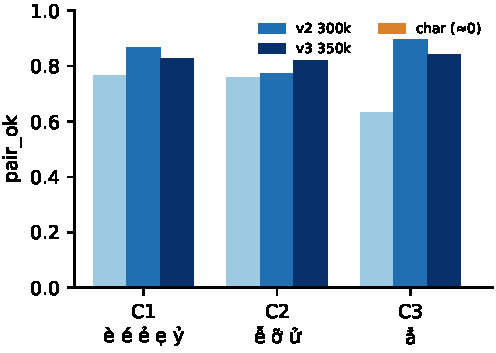
\includegraphics[width=0.55\linewidth]{heldout_groups.pdf}
\caption{\pairok{} theo nhóm ký tự giữ lại ở ba mốc. \texttt{char} xấp xỉ 0 ở mọi nhóm.}
\label{fig:heldgroups}
\end{figure}

\subsection{Ký tự đã thấy: so với VATr++}
\begin{table}[h]
\centering\small
\caption{Metric chuẩn trên 30 người viết val (2.847 từ, mỗi mô hình dùng cùng ảnh mẫu). Giá trị ``±'' là độ lệch chuẩn qua 3 seed.}
\label{tab:std}
\begin{tabular}{lcccccc}
\toprule
Mô hình & FID↓ & BFID↓ & KID$\times10^3$↓ & HWD↓ & CER↓ & Đúng cả từ↑ \\
\midrule
VATr++ VN 175,5k & 38,13 & 25,27 & 20,07 & 1,713 & 1,74\% & 94,6\% \\
VATr++ VN 250k & 38,46 & 20,77 & 21,36 & 1,613 & \textbf{1,18\%} & \textbf{96,4\%} \\
PartScribe \texttt{char} v2 300k & 16,25 & 11,62 & 5,35 & 0,871 & 2,80\% & 92,8\% \\
PartScribe \texttt{nfd} v2 300k & \textbf{16,13}±0,10 & \textbf{11,31}±0,22 & \textbf{5,31}±0,01 & 0,876±0,006 & 2,74\% & 92,7\% \\
\textbf{PartScribe \texttt{nfd} v3 350k} & 16,47 & 11,47 & 5,45 & \textbf{0,866} & 2,77\% & 92,3\% \\
\midrule
\emph{Ảnh thật} & \emph{11,9}$^\dagger$ & & & & \emph{8,80\%} & \emph{79,0\%} \\
\bottomrule
\multicolumn{7}{l}{\footnotesize $^\dagger$ FID giữa hai nửa tập ảnh thật: mức sàn thực tế với cỡ mẫu này.}
\end{tabular}
\end{table}

\begin{figure}[h]
\centering
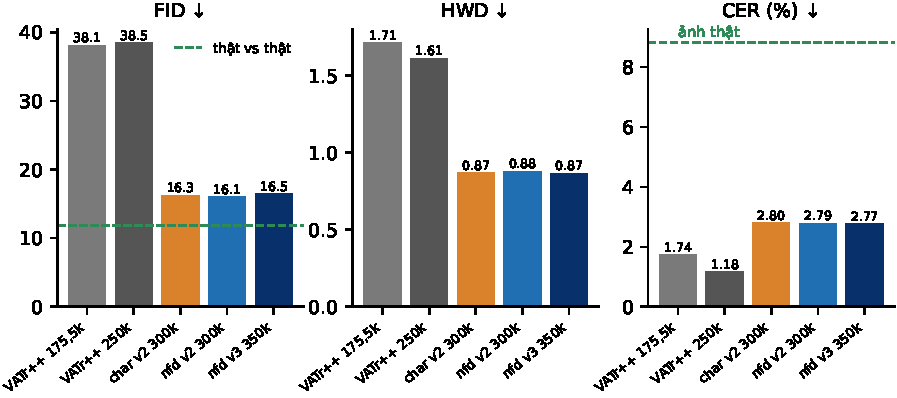
\includegraphics[width=\linewidth]{std_metrics.pdf}
\caption{FID, HWD và CER trên tập val. PartScribe giảm FID khoảng 58\% và HWD khoảng 46\% so với VATr++. CER của VATr++ thấp hơn, nhưng cả hai đều thấp hơn nhiều so với chữ thật (đường xanh lá).}
\label{fig:std}
\end{figure}

\textbf{So sánh cặp} (CI 95\% của hiệu, B $-$ A):
\begin{itemize}
\item \emph{nfd v2 300k so với VATr++ 250k}: HWD $-0{,}97..-0{,}49$, tức PartScribe giống người viết hơn rõ rệt; CER $+1{,}1..+2{,}2$ điểm \%, tức VATr++ dễ đọc hơn.
\item \emph{nfd so với char} (v2 300k): HWD và CER đều có CI chứa 0, tức \textbf{ngang nhau}. Khả năng tổ hợp không phải trả giá ở ký tự đã thấy.
\item \emph{nfd v3 350k so với nfd v2 300k}: HWD $-0{,}032..+0{,}005$, CER $-0{,}35..+0{,}30$ điểm \%, tức ngang nhau.
\end{itemize}

\note{\textbf{Vì sao CER của VATr++ thấp hơn cả ảnh thật?} VATr++ được train kèm một OCR, có loss buộc chữ phải ``đọc được''. Kết quả là chữ \emph{sạch và đều hơn chữ người thật}, nhưng kém tự nhiên và kém giống người viết (FID, HWD cao). Chữ thật có CER 8,8\% vì người thật viết ẩu, nối nét, mờ. PartScribe (2,8\%) nằm giữa: dễ đọc hơn chữ thật nhưng giữ phong cách.}

Hình~\ref{fig:vsvatr} so sánh trực quan trên các từ chọn \emph{ngẫu nhiên}. PartScribe giữ đúng \emph{cỡ chữ} của từng người: người viết nhỏ vẫn được sinh ra chữ nhỏ, trong khi VATr++ luôn kéo chữ to kín chiều cao ảnh.

\begin{figure}[h]
\centering
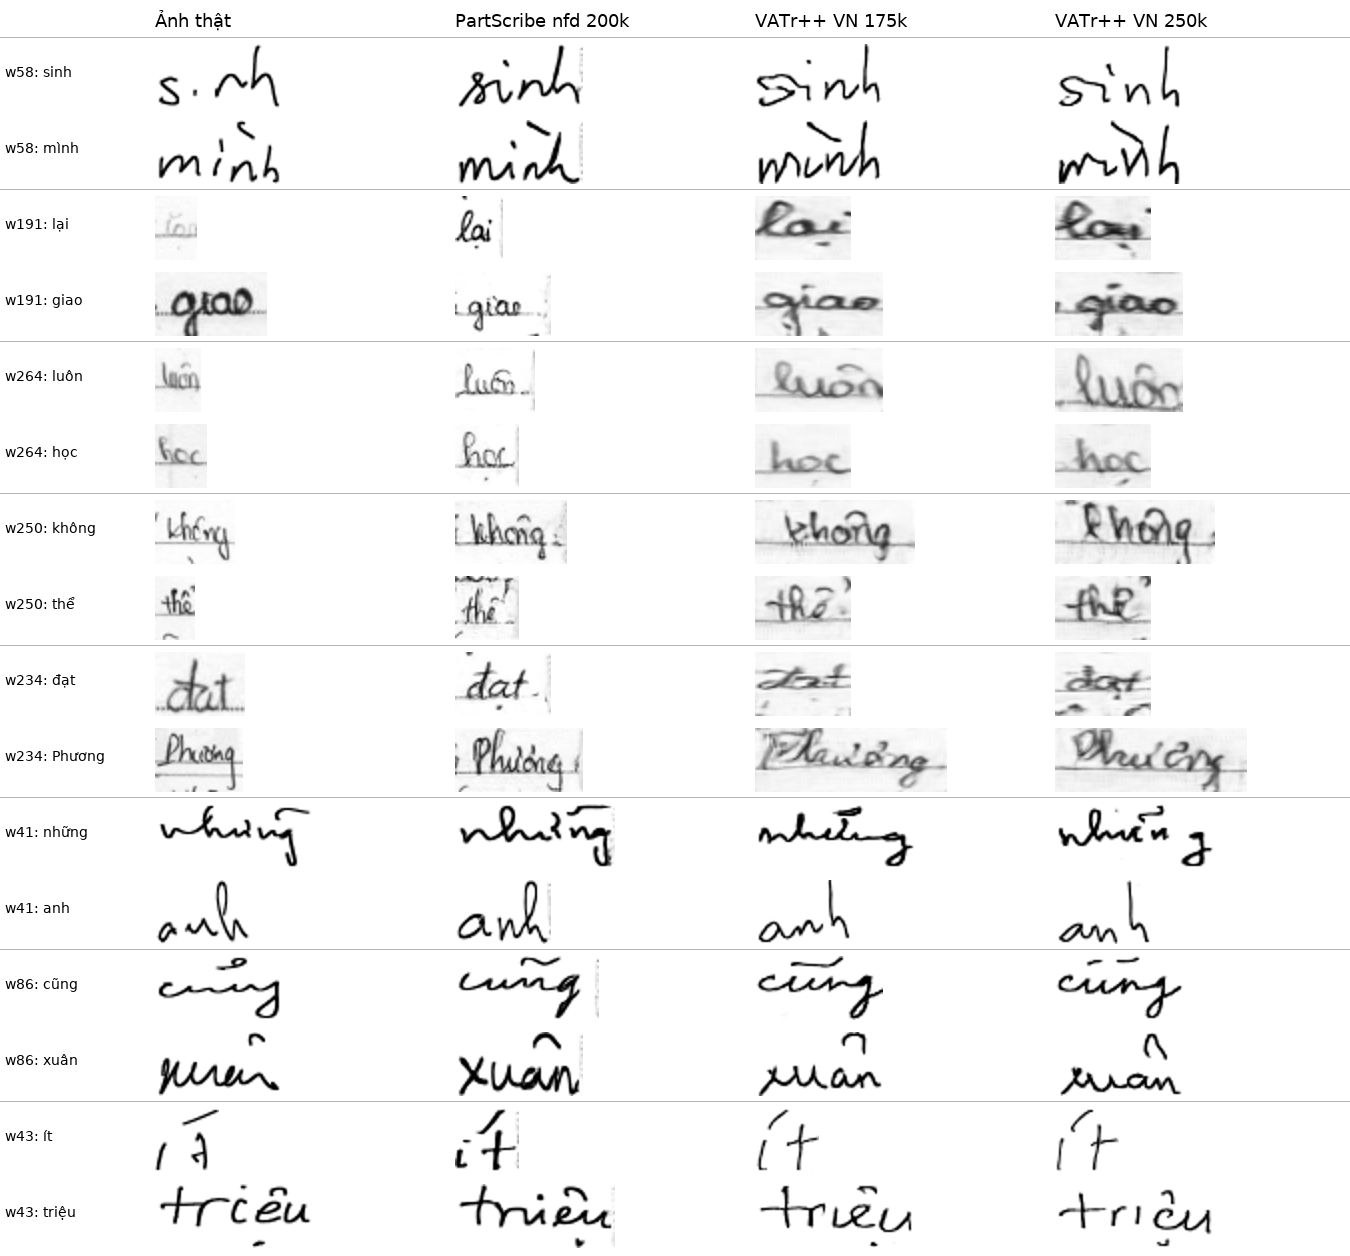
\includegraphics[width=0.85\linewidth]{best_vs_vatrpp_random.png}
\caption{Mẫu ngẫu nhiên (không chọn lọc): ảnh thật, PartScribe và VATr++ trên cùng từ, cùng người viết, cùng ảnh mẫu.}
\label{fig:vsvatr}
\end{figure}

\subsection{Chữ hoa của người viết thật (C4)}
\begin{table}[h]
\centering\small
\caption{Chữ hoa trên 5 người viết PNL không có trong train (1.653 từ). ``v2'' chưa có dữ liệu chữ hoa có người viết; ``v3'' đã có.}
\label{tab:c4}
\begin{tabular}{lccccc}
\toprule
Mô hình & FID↓ & KID$\times10^3$↓ & HWD↓ & CER↓ & Đúng cả từ↑ \\
\midrule
VATr++ VN 250k & 35,82 & 15,52 & 0,985 & 12,68\% & 64,1\% \\
\texttt{char} v2 300k & 25,98 & 12,55 & 0,828 & 8,14\% & 80,0\% \\
\texttt{nfd} v2 300k & 27,60 & 13,37 & 0,828 & 6,73\% & 84,3\% \\
\texttt{char} v3 325k & 24,69 & 12,86 & 0,697 & 6,57\% & 85,3\% \\
\texttt{nfd} v3 325k & 26,05 & 14,42 & 0,713 & \textbf{6,26\%} & \textbf{86,0\%} \\
\textbf{\texttt{nfd} v3 350k (chốt)} & 23,97 & 12,28 & 0,685 & 6,83\% & 84,9\% \\
\texttt{nfd} v3 400k & 21,79 & 9,76 & 0,619 & 6,46\% & 85,2\% \\
\texttt{char} v3 400k & \textbf{20,92} & \textbf{8,69} & \textbf{0,590} & 6,92\% & 84,4\% \\
\midrule
\emph{Ảnh thật} & \emph{15,7} & & & \emph{18,1\%}$^\ddagger$ & \emph{60,3\%} \\
\bottomrule
\multicolumn{6}{l}{\footnotesize $^\ddagger$ OCR chấm chủ yếu học chữ thường, nên đọc kém chữ hoa thật; chỉ so CER giữa các mô hình.}
\end{tabular}
\end{table}

\begin{figure}[h]
\centering
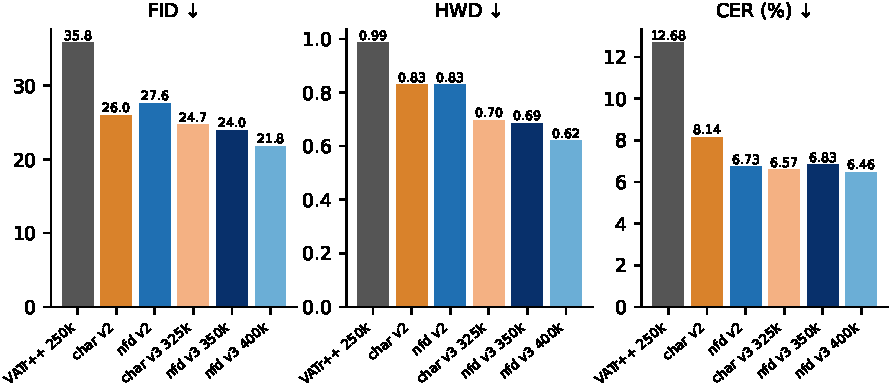
\includegraphics[width=\linewidth]{c4_metrics.pdf}
\caption{Chữ hoa trên người viết thật chưa thấy. Dữ liệu chữ hoa có người viết (v3) làm HWD giảm rõ, ở cả \texttt{char} và \texttt{nfd}.}
\label{fig:c4}
\end{figure}

\textbf{So sánh cặp:}
\begin{itemize}
\item nfd v3 350k so với nfd v2 300k: HWD $-0{,}21..-0{,}07$ (\textbf{tốt hơn, có ý nghĩa}); CER: CI chứa 0.
\item nfd v3 325k so với VATr++ 250k: HWD $-0{,}42..-0{,}15$; CER $-7{,}1..-5{,}9$ điểm \%. Trên chữ hoa, PartScribe vượt VATr++ ở \emph{cả hai} trục.
\end{itemize}
Hình~\ref{fig:names} cho ví dụ tên riêng.

\begin{figure}[h]
\centering
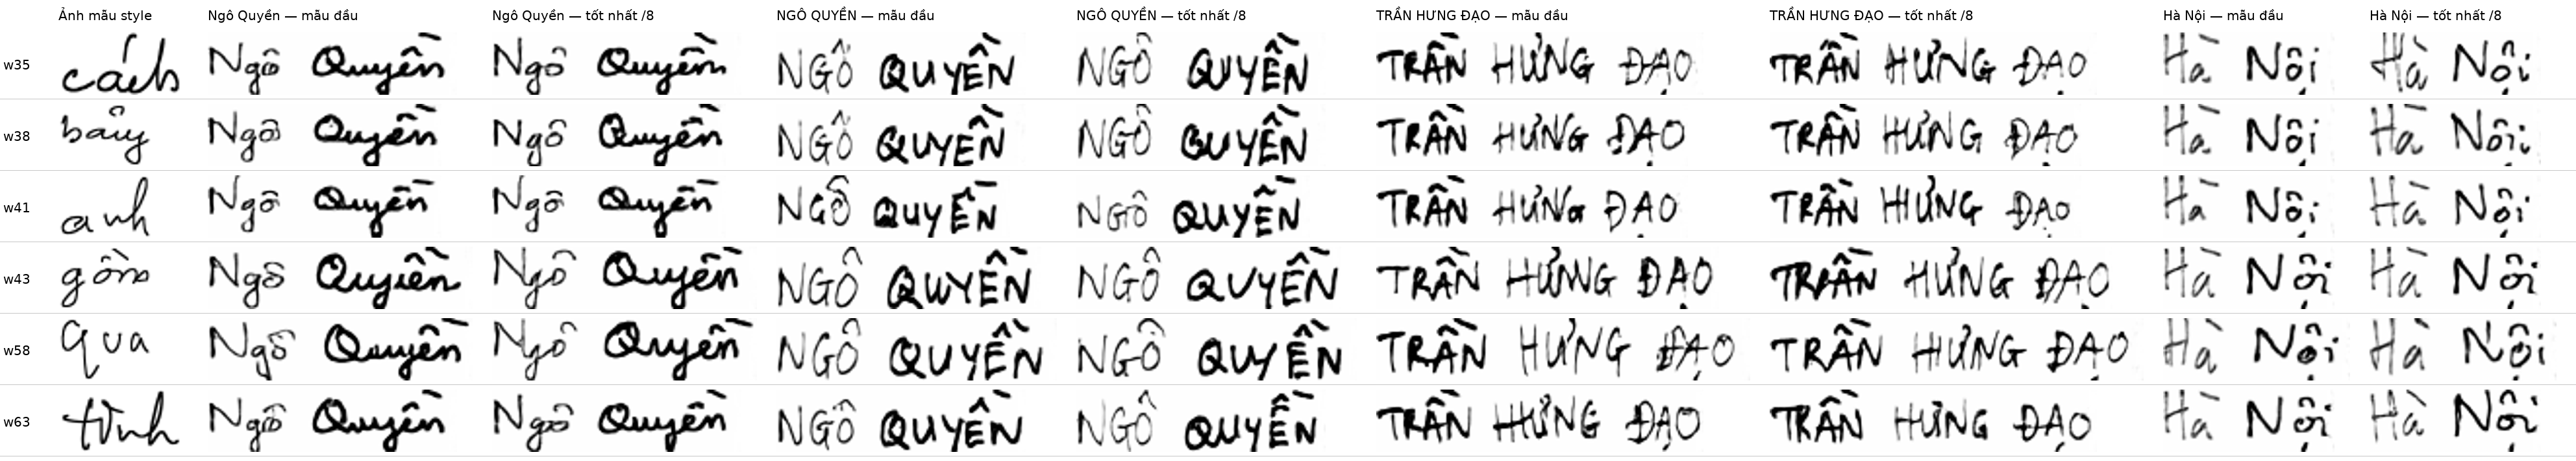
\includegraphics[width=\linewidth]{showcase_v3_350k.png}
\caption{Tên riêng do bản chốt sinh (6 người viết val). Với mỗi tên: mẫu sinh đầu tiên (không chọn lọc) và mẫu tốt nhất trong 8 lần sinh (chọn theo OCR rồi theo HWD). Chữ hoa có dấu chồng (QUYỀN, ĐẠO) đúng ở hầu hết mẫu.}
\label{fig:names}
\end{figure}

\subsection{Chọn checkpoint chốt}
\begin{table}[h]
\centering\small
\caption{Ba ứng viên trên ba trục đánh giá (val). v3 350k là điểm duy nhất không kém v2 ở trục nào.}
\label{tab:choice}
\begin{tabular}{lccc}
\toprule
Tiêu chí & v2 300k & \textbf{v3 350k} & v3 400k \\
\midrule
Ký tự giữ lại (\pairok{} C1+C2) & 0,829 & 0,823 (ngang) & 0,774 (giảm) \\
Ký tự đã thấy (CER) & 2,74\% & 2,77\% (ngang) & 3,22\% (kém hơn: CI +0,13..+0,77 điểm \%) \\
Chữ hoa (HWD) & 0,828 & 0,685 (tốt hơn) & 0,619 (tốt nhất) \\
\bottomrule
\end{tabular}
\end{table}
Train lâu hơn với dữ liệu chữ hoa làm chữ hoa tiếp tục tốt lên, nhưng khả năng tổ hợp và CER chữ thường bắt đầu giảm. Đây là dấu hiệu mô hình bắt đầu khớp quá sâu vào dữ liệu mới. Vì khả năng tổ hợp là đóng góp chính, chúng tôi chốt \textbf{v3 350k}.

\FloatBarrier
\subsection{Cấu hình sinh}
\begin{figure}[h]
\centering
\begin{minipage}{0.48\linewidth}\centering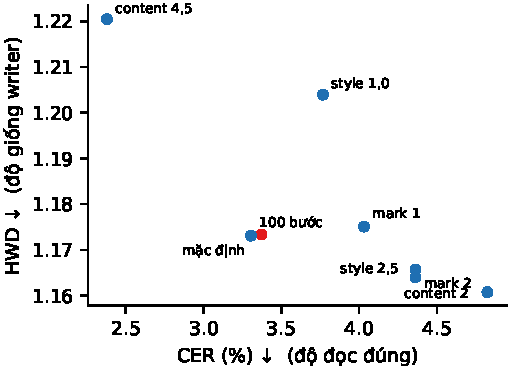
\includegraphics[width=\linewidth]{sampling_sweep.pdf}\end{minipage}\hfill
\begin{minipage}{0.5\linewidth}\footnotesize
\begin{tabular}{lcc}
\toprule
Cấu hình & HWD & CER \\
\midrule
mặc định ($w_c{=}3, w_s{=}1{,}5$) & 1,173 & 3,37\% \\
$w_c=4{,}5$ & 1,220 & \textbf{2,38\%} \\
$w_c=2$ & \textbf{1,161} & 4,82\% \\
$w_s=2{,}5$ & 1,164 & 4,36\% \\
$w_s=1{,}0$ & 1,204 & 3,77\% \\
$w_\text{mark}=1$ / $2$ & 1,175 / 1,166 & 4,03 / 4,36\% \\
100 bước & 1,173 & 3,30\% \\
\bottomrule
\end{tabular}
\end{minipage}
\caption{Quét 8 cấu hình sinh trên 450 từ val (\texttt{nfd} v2 200k, trước khi sửa mép, nên số tuyệt đối khác Bảng~\ref{tab:std}). Các cấu hình chỉ dịch chuyển giữa ``dễ đọc'' và ``giống người viết''. Guidance dấu không giúp. 100 bước không hơn 50 bước. Số báo cáo dùng cấu hình mặc định.}
\label{fig:sweep}
\end{figure}

\FloatBarrier
\subsection{Kết quả định tính}
\begin{figure}[h]
\centering
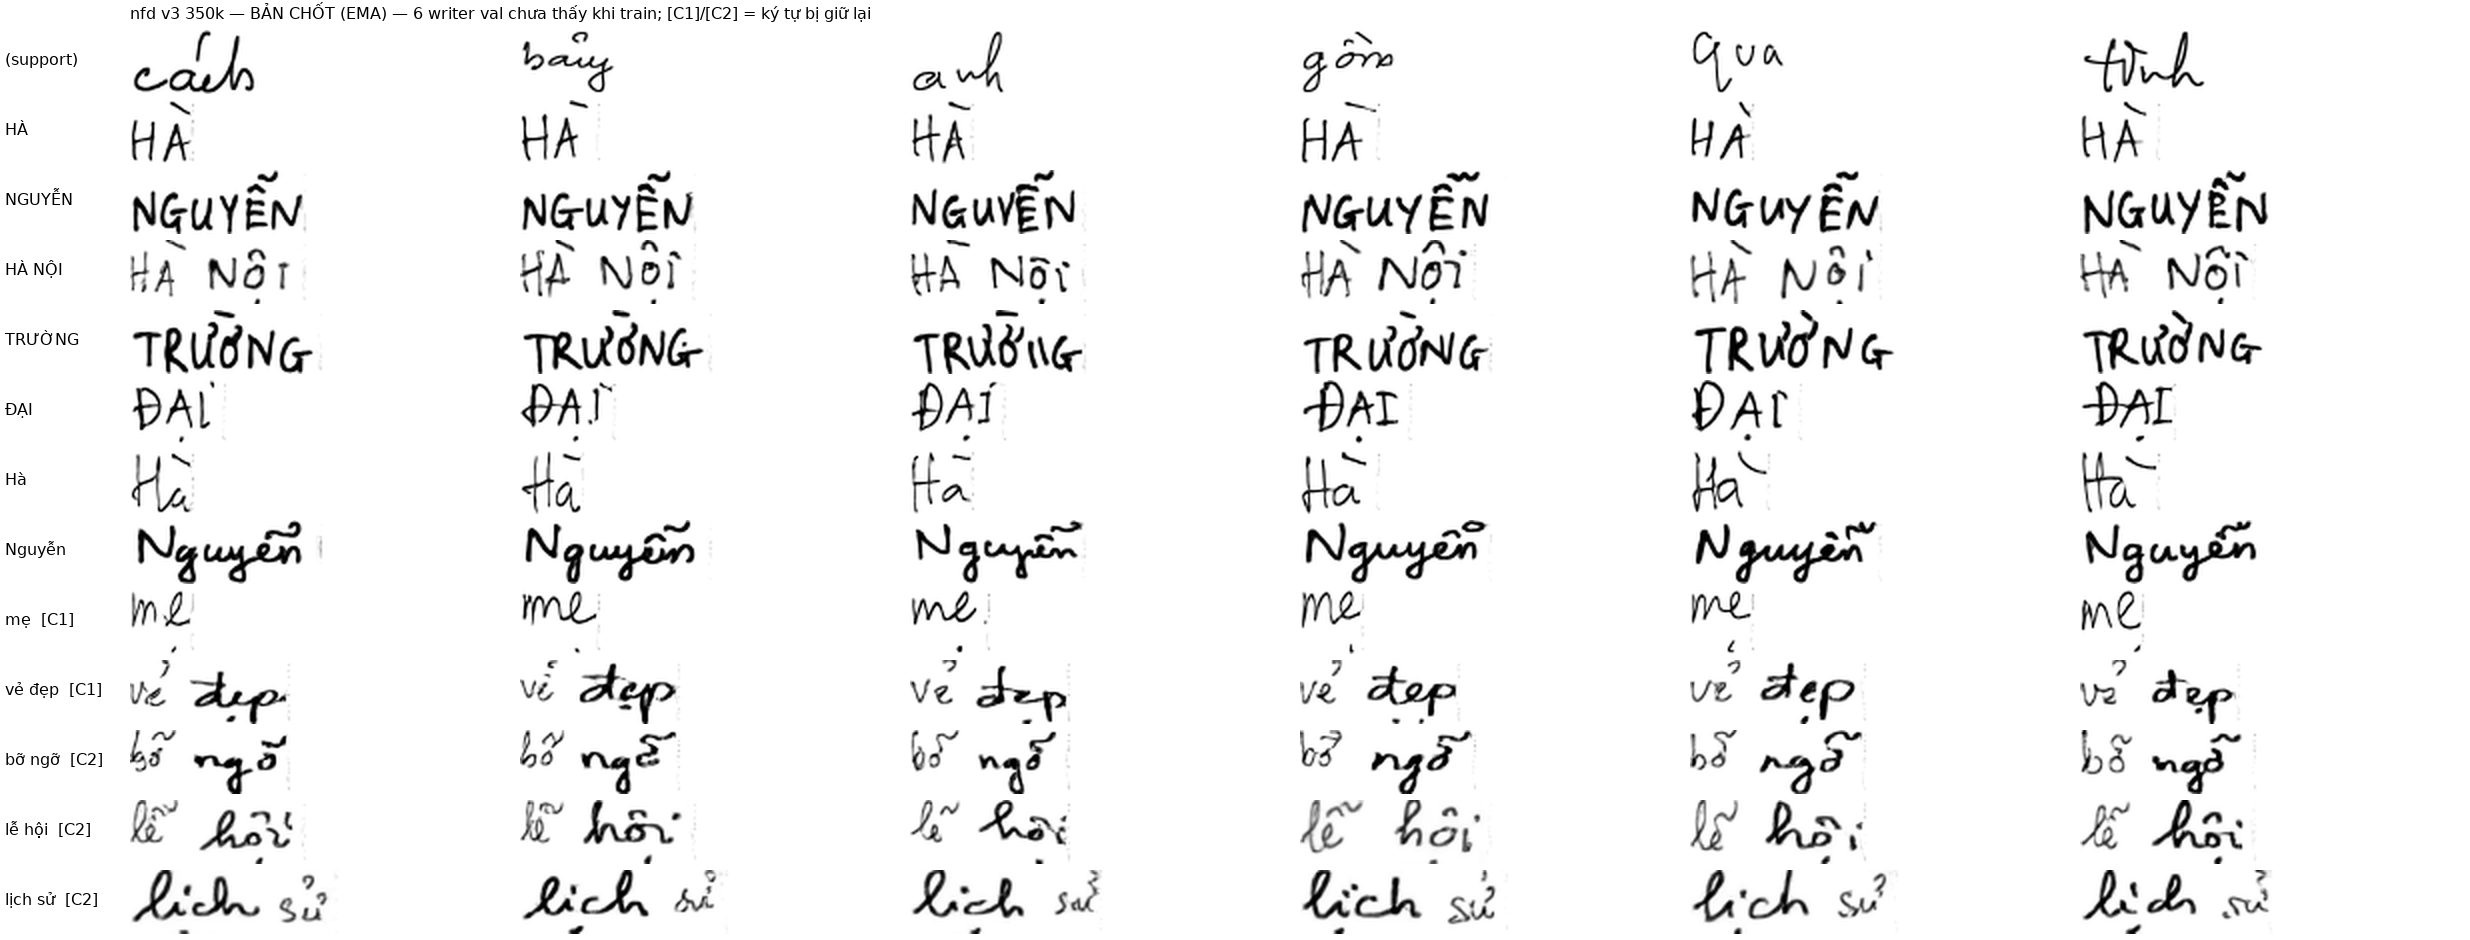
\includegraphics[width=\linewidth]{samples_nfd_v3_350k_final.png}
\caption{Bản chốt \texttt{nfd} v3 350k trên 6 người viết val (hàng đầu là một ảnh mẫu). [C1], [C2] đánh dấu từ có ký tự giữ lại.}
\label{fig:qual-nfd}
\end{figure}
\begin{figure}[h]
\centering
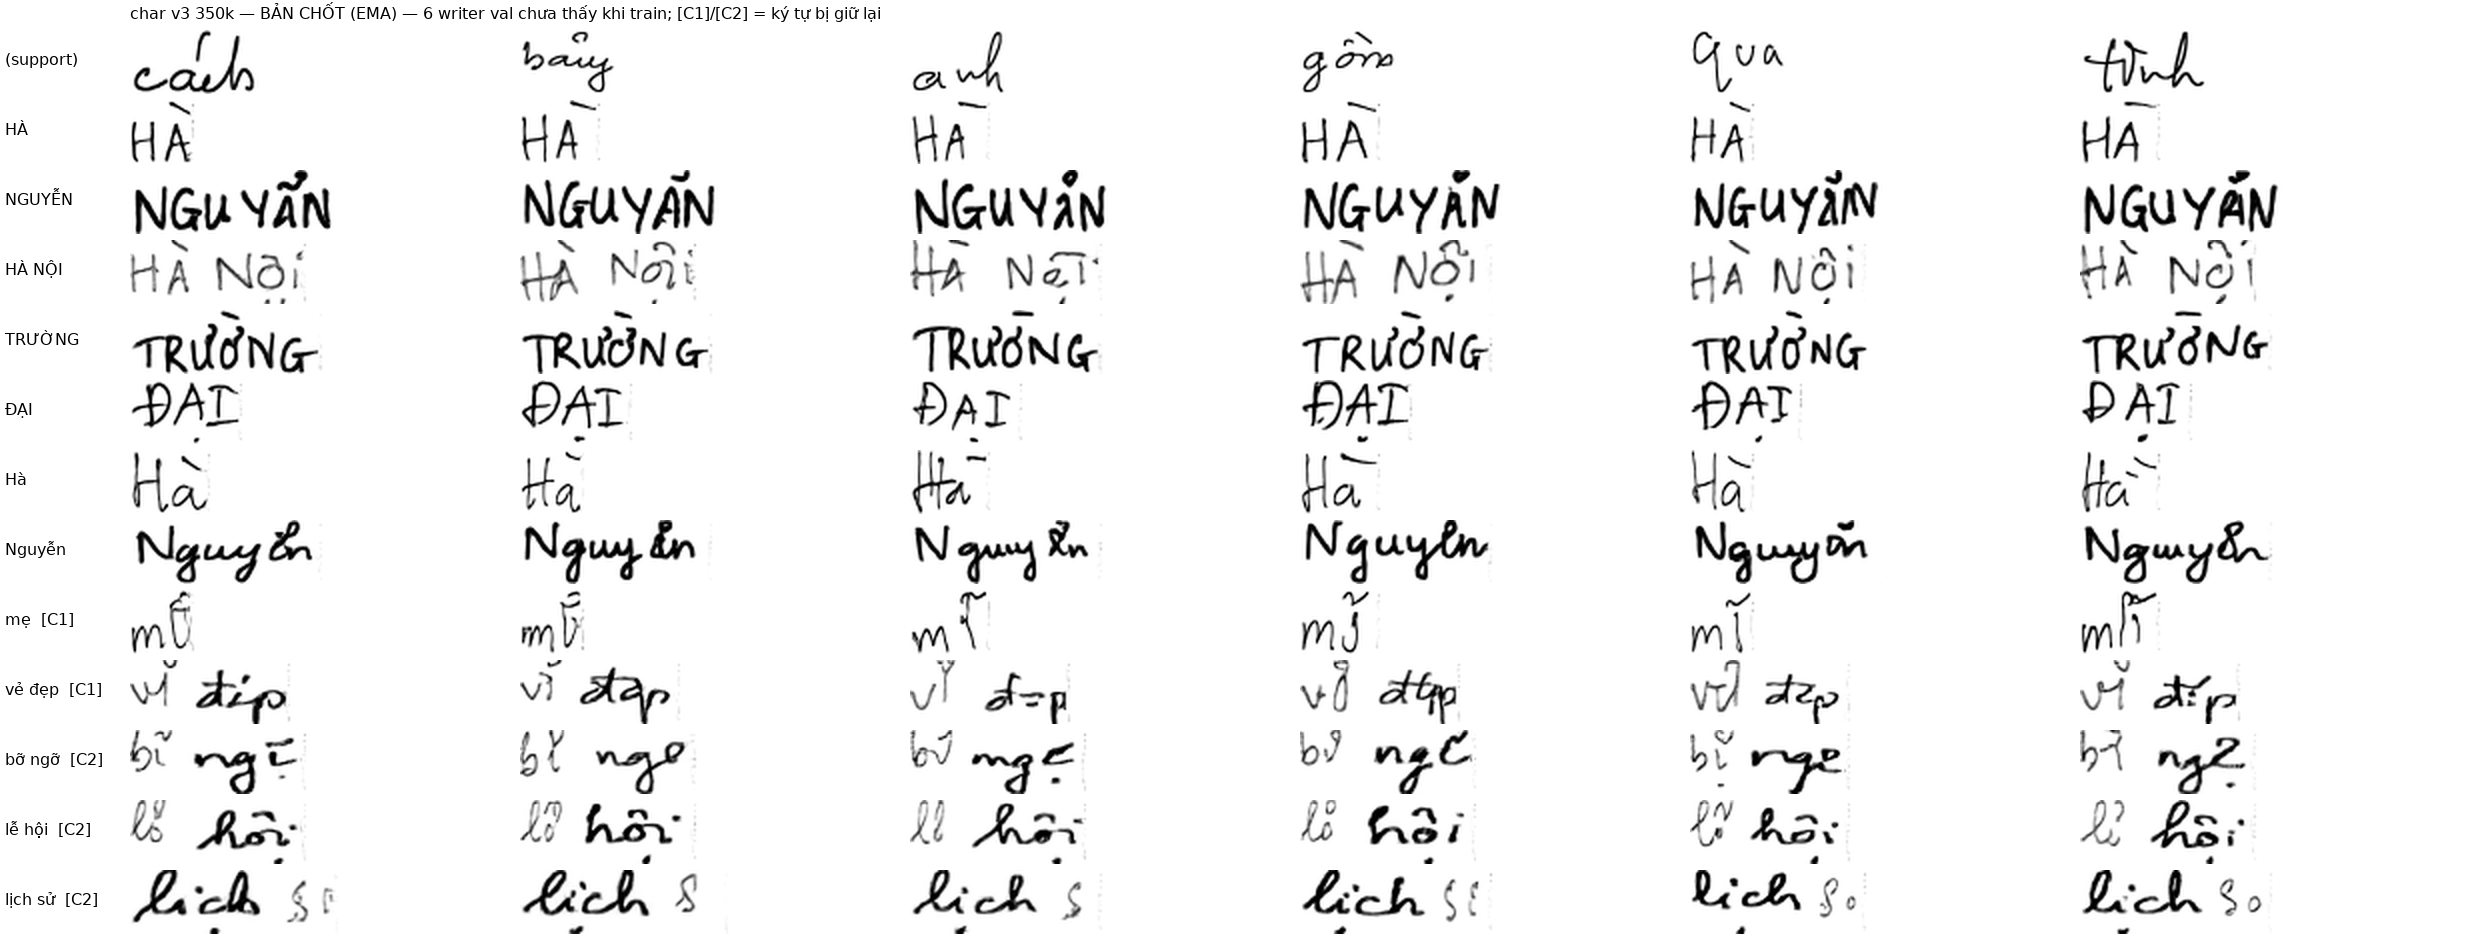
\includegraphics[width=\linewidth]{samples_char_v3_350k_final.png}
\caption{Baseline \texttt{char} v3 350k, cùng người viết và cùng từ. Chữ đã thấy được viết tốt, nhưng các ký tự giữ lại (hàng [C1], [C2]) bị thay bằng ký tự khác hoặc mất dấu.}
\label{fig:qual-char}
\end{figure}

%=====================================================================
\FloatBarrier
\section{Phân tích và thí nghiệm phụ}
\label{sec:analysis}

\subsection{Học thành phần không nhãn: kết quả null}
\label{sec:stage1}
Thiết kế ban đầu muốn học thành phần từ ảnh glyph phông chữ, \emph{không} dùng nhãn Unicode, để áp dụng được cho mọi hệ chữ. Tokenizer gồm Slot Attention (6 khe), FSQ (240 mã) và một decoder ghép các khe lại. Trước khi train generator, chúng tôi khai báo một probe kiểm tra:

\begin{center}\small
\begin{tabular}{lcccc}
\toprule
Probe & slots & global AE & pixel thô & Ngưỡng \\
\midrule
P1: đọc (thân, dấu) của ký tự giữ lại & 0,260 & 0,416 & 0,369 & slots $\ge$ global + 0,10 \\
P2: khe sở hữu dấu gọi đúng tên dấu & 0,290 & -- & 0,308 (đoán đa số) & $\ge 0{,}60$ \\
\bottomrule
\end{tabular}
\end{center}

Slot Attention \textbf{không} tách thân chữ và dấu ra các khe riêng; nó còn thua cả đặc trưng toàn cục. Theo tiêu chí đã khai báo, nhánh này bị dừng (NO-GO). Nhánh chính chuyển sang phân rã NFD, và claim ``học không nhãn'' bị bỏ. Chúng tôi báo cáo kết quả null này để người sau không lặp lại.

\subsection{Ablation cách lấy mẫu}
Ở 25k bước, lấy mẫu theo tần suất tự nhiên cho \texttt{nfd} 0,530 trên C1+C2. Long-tail sampler cho 0,756 ở 50k và 0,848 ở 75k (cùng OCR CRNN). Long-tail sampler giúp mô hình gặp các thành phần hiếm nhiều hơn, đặc biệt là các cặp dấu chồng.

\subsection{Ghép từ: căn đường chân chữ}
Ở \texttt{v2a}, mỗi từ đã được chuẩn hóa chiều cao riêng trước khi ghép. Vì vậy cụm như ``Hà Nội'' có hai từ \emph{lệch dòng và khác cỡ}, và mô hình học viết cụm từ lệch. Ở \texttt{v2}, các từ được đặt trên cùng một đường chân chữ trong một khung đủ cao, rồi thu cả dòng một lần. Mẫu ``HÀ NỘI'' sau đó cùng cỡ chữ và cùng đường kẻ.

\subsection{Vạch xám ở mép phải: nguyên nhân và cách sửa}
\label{sec:edge}
Ảnh sinh có một dải xám mờ, đều, cao hết ảnh, rộng 2--3 px ở mép phải.
\begin{itemize}
\item \textbf{Nguyên nhân}: generator đặt latent ngoài độ rộng chữ bằng 0, nhưng 0 \emph{không phải} latent của giấy trắng (latent của giấy trắng có trị tuyệt đối trung bình khoảng 0,4). Decoder vẽ bước nhảy đó thành một cạnh. Ảnh thật và latent lấy từ encoder không có hiện tượng này.
\item \textbf{Vì sao không cắt cột}: cắt bỏ cột mép sẽ cắt luôn đuôi nét chữ, vì khoảng một nửa số từ có nét chạm mép.
\item \textbf{Cách sửa}: vạch là dải đều theo chiều cao, còn nét chữ thưa và đậm. Ở 4 cột cuối, ta trừ đi \emph{trung vị theo cột}.
\item \textbf{Kết quả}: vạch biến mất (Hình~\ref{fig:edge}), 97,2\% điểm mực của nét ở mép được giữ.
\end{itemize}
Trên cùng checkpoint, các chỉ số đều tốt lên:

\begin{center}\small
\begin{tabular}{lcc}
\toprule
& Trước khi sửa & Sau khi sửa \\
\midrule
FID & 19,60 & 16,13 \\
HWD & 0,906 & 0,876 (CI hiệu $-0{,}046..-0{,}015$) \\
CER & 3,13\% & 2,74\% \\
\pairok{} & 0,793 & 0,829 \\
\bottomrule
\end{tabular}
\end{center}

BFID không đổi, đúng như dự đoán: nhị phân hóa vốn đã loại vạch mờ.

\begin{figure}[h]
\centering
\begin{minipage}{0.42\linewidth}\centering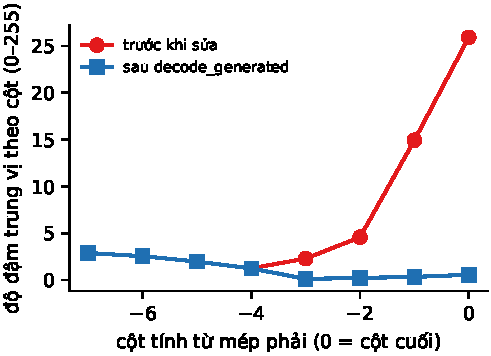
\includegraphics[width=\linewidth]{edge_profile.pdf}\end{minipage}\hfill
\begin{minipage}{0.56\linewidth}\centering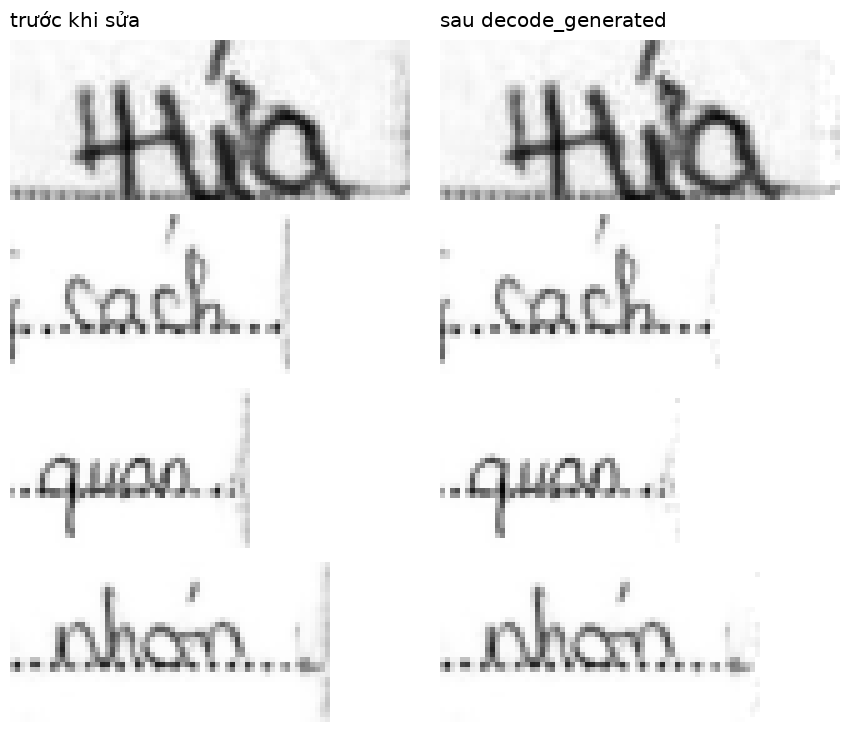
\includegraphics[width=\linewidth]{edge_zoom.png}\end{minipage}
\caption{\textbf{Trái}: độ đậm trung vị theo cột ở 8 cột cuối, trước và sau khi sửa. \textbf{Phải}: bốn từ có vạch rõ nhất, phóng to 5 lần, trước và sau khi sửa (cùng checkpoint, cùng nhiễu); chú ý cột xám ở mép phải.}
\label{fig:edge}
\end{figure}

\subsection{Hội tụ}
Từ 100k đến 300k bước, flow loss giảm đều. Các chỉ số trên tập val bão hòa sớm hơn:

\begin{center}\small
\begin{tabular}{lcc}
\toprule
Chỉ số & Trạng thái & Từ mốc \\
\midrule
FID & đi ngang (19,6 ở cả 200k và 300k, trước khi sửa mép) & khoảng 200k \\
HWD & đi ngang (0,91--0,92) & khoảng 125k \\
CER & còn giảm nhẹ (3,32\% → 3,13\%) & -- \\
\pairok{} & dao động trong CI & khoảng 200k \\
\bottomrule
\end{tabular}
\end{center}

Loss train giảm nhưng chỉ số val không đổi cho thấy phần giảm loss chủ yếu là khớp sâu hơn vào dữ liệu train.

%=====================================================================
\FloatBarrier
\section{Giới hạn và lỗi còn lại}
\label{sec:limits}
\begin{enumerate}
\item \textbf{Dấu nặng của \emph{ẹ} (ký tự giữ lại) thường bị mất.} Dấu chấm chỉ rộng vài pixel và nằm sát mép dưới khung 32 px. Với ký tự đã thấy, \texttt{char} vẽ chấm dưới chắc hơn \texttt{nfd}. Thêm dữ liệu chữ hoa cải thiện chấm dưới trên Ạ, Ộ. Guidance dấu không sửa được.
\item \textbf{Tên riêng viết thường có chữ hoa đầu từ} (``Ngô Quyền'', ``Trần Hưng Đạo'') ra gần như cùng một kiểu chữ đậm cho mọi người viết. Giả thuyết: dữ liệu HAT2023, vốn nhiều tên riêng, được train \emph{không kèm phong cách}, nên mô hình gắn loại văn bản này với một kiểu chữ chung. Chữ hoa toàn bộ cũng kém đa dạng hơn chữ hoa thật.
\item \textbf{Tiếng Anh (IAM) chưa có kết quả}; chưa có bảng so sánh chuẩn với các công trình khác.
\item \textbf{Chưa có VATr++ train lại dưới cùng protocol.} VATr++ hiện có đã thấy các ký tự giữ lại, nên chưa so sánh được trên \pairok{}.
\item \textbf{Mẫu nhỏ}: C3 có 11 người viết; tập chữ hoa có 5 người viết.
\item \textbf{Mọi số liệu đo trên tập val}, cũng là tập dùng để chọn checkpoint. Tập test VN vẫn niêm phong.
\end{enumerate}

%=====================================================================
\section{Tái lập}
\label{sec:repro}

\begin{table}[h]
\centering\small
\caption{Checkpoint giữ lại (thư mục \texttt{runs/}).}
\label{tab:ckpt}
\begin{tabularx}{\linewidth}{lX}
\toprule
Đường dẫn & Vai trò \\
\midrule
\texttt{gen\_vn\_\{nfd,char\}\_v3/snap\_350000.pt} & \textbf{Bản chốt} (chỉ đọc). SHA-256 nfd \texttt{f3830dc2\dots}, char \texttt{819fd211\dots} \\
\texttt{gen\_vn\_\{nfd,char\}\_v3/snap\_400000.pt} & Mốc cuối v3 \\
\texttt{gen\_vn\_\{nfd,char\}\_v2/snap\_300000.pt} & Bản chốt trước \\
\texttt{gen\_vn\_\{nfd,char\}\_lt/snap\_100000.pt} & Điểm khởi tạo của v2 \\
\texttt{vae\_vn32/final.pt} & VAE 32 px \\
\texttt{eval\_ocr\_vn/best.pt}, \texttt{eval\_ocr\_vn\_local/best.pt} & OCR chấm CER; LocalOCR chấm \pairok{} \\
\bottomrule
\end{tabularx}
\end{table}

\paragraph{Lệnh chính} (thư mục \texttt{hand\_writting/PartScribe}):
{\footnotesize
\begin{verbatim}
bash scripts/pipeline.sh gen_nfd_v2
bash scripts/pipeline.sh gen_nfd_v2_300k
python scripts/prepare_pnl.py --release <handwriting_word_v1.0> \
    --out data/pnl32.npz
bash scripts/pipeline.sh gen_nfd_v3
python scripts/eval_holdout.py run \
    --ckpt runs/gen_vn_nfd_v3/snap_350000.pt --vae runs/vae_vn32/final.pt \
    --ocr runs/eval_ocr_vn_local/best.pt --raw --pairs --out r.json
python scripts/eval_standard.py {jobs|partscribe|vatr|score|paired} \
    [--pool pnl_test] --out <dir> --hwd-repo <clone of aimagelab/HWD>
python paper/make_figures.py && python paper/make_gen_figures.py
\end{verbatim}}
Tài liệu đi kèm:
\begin{itemize}
\item số liệu chốt: \texttt{docs/final\_v3\_350k.json};
\item diễn biến chi tiết: \texttt{docs/261122\_report\_01\_*.md}.
\end{itemize}

%=====================================================================
\section{Kết luận}
PartScribe cho thấy, trên tiếng Việt, \textbf{biểu diễn nội dung bằng thành phần dùng chung} cho phép một mô hình sinh chữ viết tay \textbf{viết đúng các ký tự chưa từng có ảnh} khi train:
\begin{itemize}
\item \pairok{} 0,82 so với gần 0 của biểu diễn nguyên khối, trên cùng kiến trúc và dữ liệu;
\item \emph{không} làm giảm chất lượng trên ký tự đã thấy;
\item vượt VATr++ rõ rệt về độ giống ảnh thật và độ giống người viết.
\end{itemize}
Bổ sung dữ liệu chữ hoa có người viết thật làm chữ hoa giống người viết hơn nhiều.

Các bước tiếp theo:
\begin{itemize}
\item mở tập test;
\item train lại VATr++ dưới cùng protocol;
\item sửa dấu chấm dưới và tính đa dạng của chữ hoa;
\item kiểm tra trên tiếng Anh (IAM).
\end{itemize}

%=====================================================================
\begin{thebibliography}{99}\small
\bibitem{vaswani2017} A. Vaswani et al. Attention is all you need. NeurIPS 2017.
\bibitem{peebles2023} W. Peebles, S. Xie. Scalable diffusion models with transformers (DiT). ICCV 2023.
\bibitem{kingma2014} D. P. Kingma, M. Welling. Auto-encoding variational Bayes. ICLR 2014.
\bibitem{rombach2022} R. Rombach et al. High-resolution image synthesis with latent diffusion models. CVPR 2022.
\bibitem{ho2020} J. Ho, A. Jain, P. Abbeel. Denoising diffusion probabilistic models. NeurIPS 2020.
\bibitem{liu2023flow} X. Liu, C. Gong, Q. Liu. Flow straight and fast: learning to generate and transfer data with rectified flow. ICLR 2023.
\bibitem{lipman2023} Y. Lipman et al. Flow matching for generative modeling. ICLR 2023.
\bibitem{esser2024} P. Esser et al. Scaling rectified flow transformers for high-resolution image synthesis (SD3). ICML 2024.
\bibitem{ho2022cfg} J. Ho, T. Salimans. Classifier-free diffusion guidance. NeurIPS Workshop 2021 / arXiv 2022.
\bibitem{heusel2017} M. Heusel et al. GANs trained by a two time-scale update rule converge to a local Nash equilibrium (FID). NeurIPS 2017.
\bibitem{binkowski2018} M. Bińkowski et al. Demystifying MMD GANs (KID). ICLR 2018.
\bibitem{pippi2023hwd} V. Pippi, F. Quattrini, S. Cascianelli, R. Cucchiara. HWD: a novel evaluation score for styled handwritten text generation. BMVC 2023.
\bibitem{bhunia2021hwt} A. K. Bhunia et al. Handwriting transformers. ICCV 2021.
\bibitem{pippi2023vatr} V. Pippi, S. Cascianelli, R. Cucchiara. Handwritten text generation from visual archetypes (VATr). CVPR 2023.
\bibitem{vanherle2024vatrpp} B. Vanherle, V. Pippi, S. Cascianelli et al. VATr++: choose your words wisely for handwritten text generation. arXiv 2024.
\bibitem{nikolaidou2024} K. Nikolaidou et al. DiffusionPen: towards controlling the style of handwritten text generation. ECCV 2024.
\bibitem{dai2024onedm} G. Dai et al. One-DM: one-shot diffusion mimicker for handwritten text generation. ECCV 2024.
\bibitem{pippi2025emuru} V. Pippi et al. Zero-shot styled text image generation, but make it autoregressive (Emuru). CVPR 2025.
\bibitem{inkspire2026} Wang, Zhang, Yao, Yin, Liu. InkSpire. ICLR 2026.
\bibitem{dai2023sdt} G. Dai et al. Disentangling writer and character styles for handwriting generation (SDT). CVPR 2023.
\bibitem{khosla2020} P. Khosla et al. Supervised contrastive learning. NeurIPS 2020.
\bibitem{ganin2015} Y. Ganin, V. Lempitsky. Unsupervised domain adaptation by backpropagation. ICML 2015.
\bibitem{shi2017crnn} B. Shi, X. Bai, C. Yao. An end-to-end trainable neural network for image-based sequence recognition (CRNN). TPAMI 2017.
\bibitem{locatello2020} F. Locatello et al. Object-centric learning with slot attention. NeurIPS 2020.
\bibitem{mentzer2024} F. Mentzer et al. Finite scalar quantization: VQ-VAE made simple. ICLR 2024.
\end{thebibliography}

%=====================================================================
\appendix
\section{Bảng siêu tham số đầy đủ}
\begin{table}[H]
\centering\footnotesize
\resizebox{\linewidth}{!}{%
\begin{tabular}{llll}
\toprule
Nhóm & Tham số & Giá trị & Ghi chú \\
\midrule
VAE & hệ số nén $f$, kênh latent & 4, 4 & ảnh 32 px $\to$ latent $4\times8\times W/4$ \\
& loss & L1 + 1,0·Sobel + $10^{-6}$·KL + 0,05·PatchGAN & GAN từ bước 20k \\
& bước, batch, lr & 100k, 64, $2\cdot10^{-4}$ & \\
Nội dung & chế độ, chiều, lớp & \texttt{nfd}, 384, 4 lớp × 6 đầu & tối đa 3 token/ký tự \\
Phong cách & ảnh mẫu, rộng & 15, 192 px & 4 query cho $g$ \\
DiT & block, chiều, đầu, patch & 8, 384, 6, $2\times2$ & cổng khởi tạo 0 \\
Loss & độ rộng, SupCon, chống nội dung & 0,1; 0,05; 0,05 & SupCon $\tau=0{,}1$ \\
CFG dropout & nội dung, phong cách & 0,1; 0,1 & \\
Tối ưu & AdamW, lr, warmup, wd & $10^{-4}$, 5k, 0,01 & lr cố định; clip 1,0; bf16 \\
EMA & decay & 0,9999 & có khởi động \\
Batch & người viết × ảnh & 16 × 4 (+16 HAT) & \\
Lấy mẫu & long-tail, trộn thành phần & 0,3; 0,5 & theo VATr-pp \\
& multiword, trọng số dấu, PNL & 0,2; 3; 0,15 & PNL chỉ ở v3 \\
Sinh & bước Euler, $w_c$, $w_s$ & 50, 3,0, 1,5 & \\
\bottomrule
\end{tabular}}
\end{table}

\section{Bảng thuật ngữ}
\begin{table}[H]
\centering\small
\begin{tabularx}{\linewidth}{lX}
\toprule
Thuật ngữ & Giải thích ngắn \\
\midrule
HTG & Handwritten Text Generation: sinh ảnh chữ viết tay \\
Support & Các ảnh mẫu của người viết, dùng để lấy phong cách \\
Latent & Biểu diễn nén của ảnh do VAE tạo ra \\
Rectified flow & Mô hình sinh học vận tốc dọc đường thẳng nối nhiễu và dữ liệu \\
DiT & Transformer dùng để khử nhiễu ảnh, ảnh được cắt thành patch \\
CFG & Classifier-free guidance: khuếch đại ảnh hưởng của điều kiện khi sinh \\
NFC / NFD & Hai dạng chuẩn hóa Unicode: ký tự liền / tách chữ gốc + dấu tổ hợp \\
Embedding & Vector học được đại diện cho một ký hiệu rời rạc \\
EMA & Trung bình trượt của trọng số, cho mô hình mượt và ổn định hơn \\
\pairok & Chỉ số đúng có đối chứng: có dấu đọc đúng, bỏ dấu thì không đọc ra \\
FID / KID / BFID & Khoảng cách phân bố giữa ảnh thật và ảnh sinh (BFID: trên ảnh nhị phân) \\
HWD & Khoảng cách phong cách chữ viết, tính theo từng người viết \\
CER & Tỉ lệ lỗi ký tự khi OCR đọc ảnh \\
CI 95\% & Khoảng tin cậy 95\%, ở đây tính bằng bootstrap theo người viết \\
\bottomrule
\end{tabularx}
\end{table}

\section{Hình bổ sung}
\begin{figure}[H]
\centering
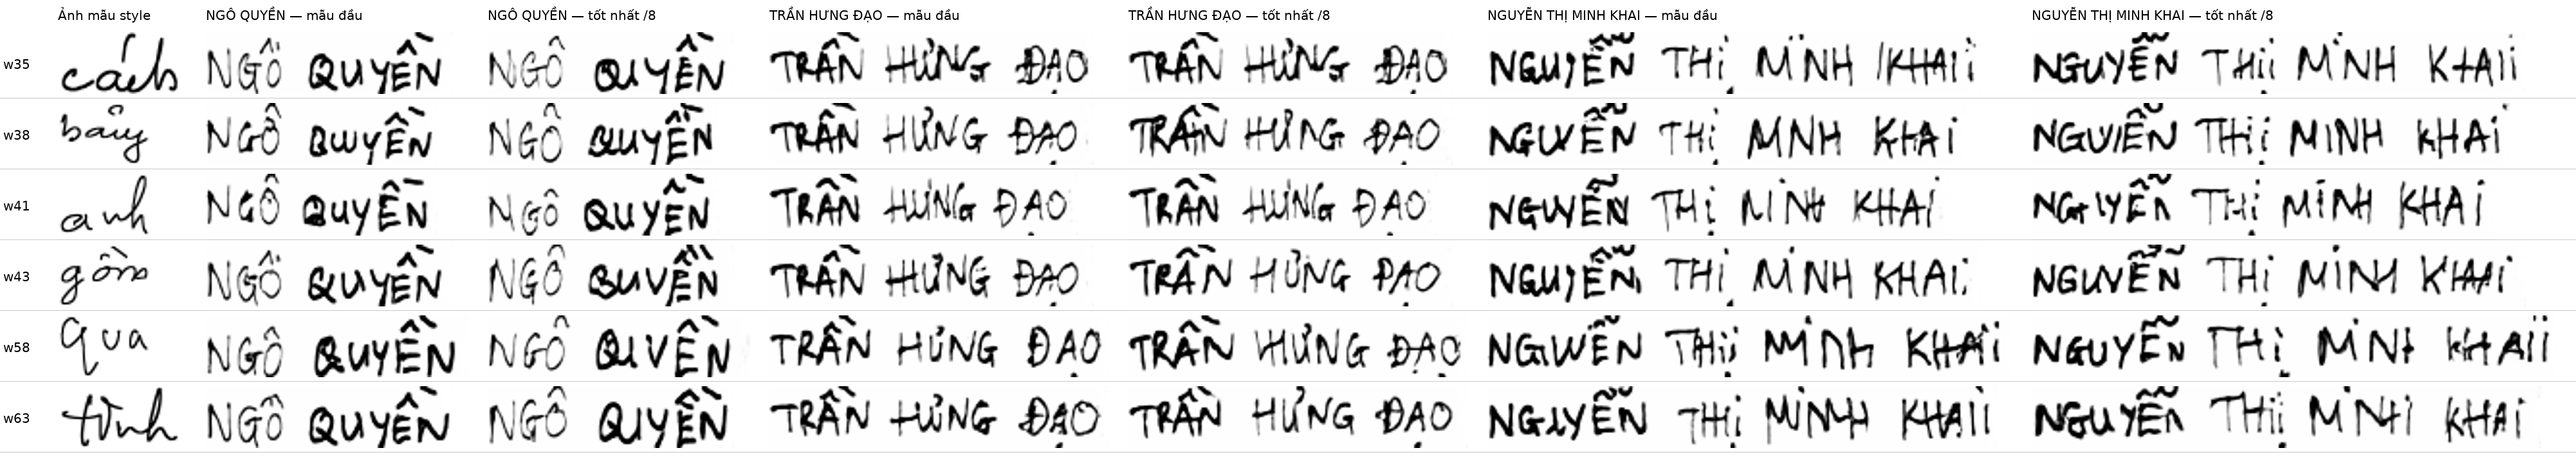
\includegraphics[width=\linewidth]{names_upper_v2.png}\\[3pt]
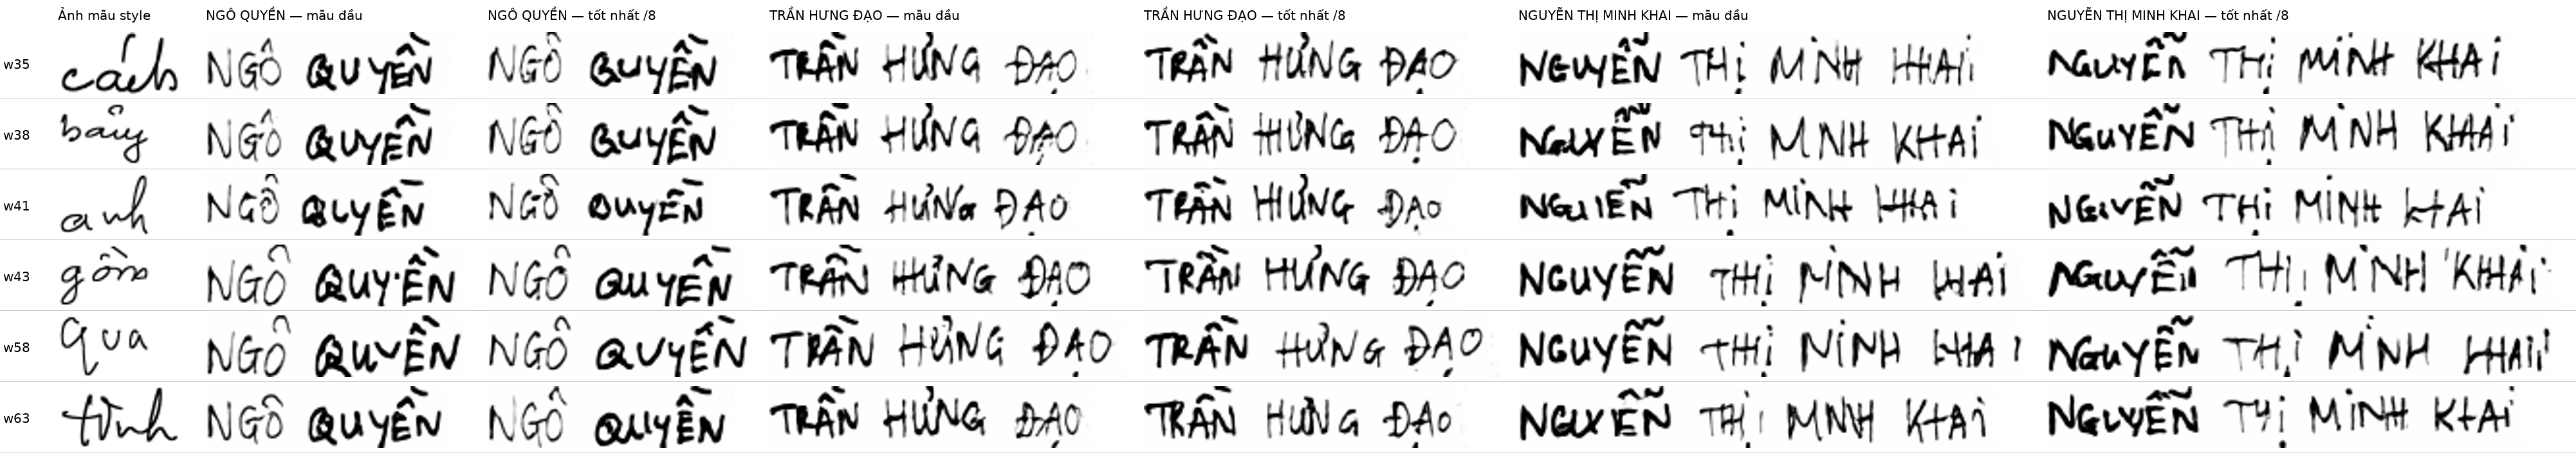
\includegraphics[width=\linewidth]{names_upper_v3.png}
\caption{Tên viết hoa trước (trên, v2 300k) và sau (dưới, v3 375k) khi thêm dữ liệu chữ hoa có người viết.}
\end{figure}

\end{document}
